\documentclass{article}
\usepackage{iclr2026_conference}
\usepackage{fontspec}
\usepackage{xeCJK}
\usepackage{amsmath,amssymb}
\usepackage{booktabs}
\usepackage{tabularx}
\usepackage{graphicx}
\usepackage{hyperref}
\usepackage{url}

\setmainfont{Latin Modern Roman}
\setCJKmainfont{Noto Serif CJK SC}
\setCJKsansfont{Noto Sans CJK SC}
\setCJKmonofont{Noto Sans CJK SC}

\title{中文场景下记忆冲突的可信度裁决：贝叶斯框架与中文语用信号的实证研究}
\author{}  % 匿名投稿；camera-ready 时填写作者信息并取消注释 \iclrfinalcopy
%\iclrfinalcopy
\begin{document}
\maketitle

\begin{abstract}
长期运行的 AI agent 记忆中常出现针对同一事实的矛盾说法，但主流系统仅以时间新近性（last-write-wins）或临时性的 LLM 临场判断来裁决。英文中已有可信度条件贝叶斯裁决的探索\citep{singh2026}，但其能否迁移到中文——中文的认识情态、语域与指代消解行为均与英文不同——尚未被检验。本文首次对中文场景下的可信度记忆冲突裁决开展实证研究。我们构建了 240 条中文冲突评测集，对齐 LongMemEval 题型分类，其中 45\% 为"旧说法更可信"的对抗样本，可把可信度裁决与新近性启发式区分开。我们将中文语用信号——三级模糊限制语强度、语域、指代风险——形式化为三元组可信度模型（来源类型先验、语用特征、佐证计数）的可靠性特征，配合贝叶斯后验裁决、来源上限与影子证据审计。我们复现了 4 个基线（含去掉英文专属组件的英文贝叶斯方法），并设计消融实验分离各中文信号的边际贡献，以及规则检测 vs LLM 检测的成本-准确率对比（对应 RQ1–RQ3）。本文的贡献为：(1) 首个中文可信度裁决实证研究及其适用边界；(2) 中文特有可信度信号的形式化与消融；(3) 公开的中文冲突评测集；(4) 跨语言基线复现，回答"英文强的方法中文是否依然强"。确定性方法已真实运行（n=240）：本方法准确率 1.0000 [0.9842, 1.0000]，对抗子集 108/108 全对、误覆盖率 0；英文贝叶斯基线（Nous 复现）0.9833，与本方法的差距经 McNemar 检验不显著（p=0.125）；last-write-wins 在对抗子集上 0/108、误覆盖率 1.0000。消融显示中文信号整体贡献 +30.00pp（$p=4.2\times 10^{-22}$），其中模糊限制语强度主导（+13.33pp），语域呈冗余-互补模式；佐证计数在当前数据上不可识别。LLM 方法已用 DeepSeek 真实调用补齐：纯 LLM zero-shot 准确率 0.9625（9 条错误全是对抗样本，显著弱于本方法，p=0.0039），Ours+LLM 检测与规则检测版逐条一致（1.0000），240 次调用约 4.8 万真实 token 未带来任何增益。鲁棒性分析显示 24 个主题全部满分、17 组权重扰动下准确率恒定：结果不依赖个别主题或参数初值，但也反证合成数据信号可分性过强，生态效度见第 6 章讨论。
\end{abstract}

\section{引言}

长期运行的 AI agent 需要在多会话、跨时间的交互中保持记忆连贯。伴随着记忆的写入，同一事实却常常出现矛盾说法：用户改口、转述他人之言、agent 误记、工具返回结果与文档记录互相冲突。如何裁决这些冲突，将直接决定 agent 回答的可信度，也决定用户是否敢把重要事项托付给 agent。


现有系统大多采用两种粗糙策略。\textbf{时间最新者胜}（last-write-wins）：如 Mem0 v3 的单遍 ADD-only 机制，冲突靠后写覆盖解决。该策略隐含"新说法更可信"的假设，但是在"旧说法更可信"的场景下会犯错——例如用户随口一说覆盖了此前有官方文件支撑的记录。\textbf{LLM 临场判定}：如 Zep/Graphiti 的矛盾边失效判定（新边与旧边时间重叠且矛盾时，置旧边失效），把裁决交给 LLM 的即时判断，没有对"可信度"做显式建模，裁决过程不可审计、不可复现。值得注意的是，Zep 的双时态机制解决的是"何时为真"（$t_{\mathrm{valid}}/t_{\mathrm{invalid}}$），并不解决"有多可信"；而它在 knowledge-update 上的自报分数（83.3\%）反而不如 Mem0 ADD-only（93.6\%），说明机制复杂度不等于裁决收益。


英文文献中已有可信度裁决方向的探索。Nous\citep{singh2026}提出 reliability-conditional Bayesian updating：每个 $(entity, attribute)$ 维护取值的分类概率分布，以贝叶斯后验做冲突裁决，可靠性从 epistemic markers 估计，并以 provenance cap（$\mathrm{trust}=\min(\mathrm{provenance},\mathrm{content})$）防范措辞操纵。BeliefMem\citep{liao2026}用 Noisy-OR 规则合并多候选信念。MemoryMesh 等开源工程则用 Beta-Bernoulli 后验维护来源信任。但这些工作\textbf{只覆盖英文}：Nous 的可靠性估计依赖英文 epistemic markers 词表（maybe / I think / actually / definitely），其实测数据是英文模板合成的，provenance 等级由 oracle 指派。


中文场景带来了英文研究未曾面对的变量。中文认识情态有独立的三级强度体系\citep{jia2023}；"可能"在新闻标题与网络口语中还存在非推测性用法（提醒、调侃、弱化语气），并不表达真正的不确定性；"听说/据说"这类传信标记同时承载证据来源信息；口语转述与正式陈述的语域差异会影响 hedge 的分布；"老王/王总/他"这类指代需要正确消解才能确定主张的归属。这些因素会不会让英文验证过的方法失效、会不会带来新的失效模式——\textbf{尚未被检验}。


与此同时，中文评测资源存在明确空白。PerLTQA\citep{du2024}是中文个性化长期记忆 QA 基准（8,593 问题 / 30 角色），但其任务定义中没有冲突来源可靠性标注、不测可信度冲突消解，也不直接评测完整的 agent 记忆系统本身。LongMemEval\citep{wang2024}的 knowledge-update 子集（78 题）测的是"同一事实随时间变化$\to$返回最新版本"的 recency 语义，而非"来源可信度不同"情况下的冲突裁决，且 N=78 统计效力弱。中文 agent 记忆评测基准整体缺失，这正是本研究自建中文冲突数据集的正当性依据。


本研究定位为\textbf{工程实证型}：不以发明全新方法为核心卖点，而是检验已有可信度裁决范式在中文语境下的适用边界，回答三个研究问题：


\begin{itemize}
\item \textbf{RQ1}：英文验证过的可信度裁决方法迁移到中文个人助理记忆场景后，准确率是否保持？哪些失效模式是中文特有的？
\item \textbf{RQ2}：中文语用信号——模糊限制语强度、语域差异、指代消解正确性——能否作为可信度特征显式建模，并带来可测量的准确率提升？
\item \textbf{RQ3}：确定性规则检测 vs LLM 判断式检测的成本-准确率权衡曲线，在中文语料上是否与英文文献结论一致？
\end{itemize}

本文的四个贡献点是：


\begin{enumerate}
\item \textbf{首个针对中文场景的记忆冲突可信度裁决实证研究}：检验 reliability-conditional 贝叶斯裁决范式在中文语境下的适用边界，定位中文特有的失效模式。
\item \textbf{中文特有可信度信号的形式化与消融}：将模糊限制语强度三档、语域、指代消解正确性纳入可信度特征，量化各自的边际贡献。
\item \textbf{配套中文评测集}：240 条中文冲突数据，对齐 LongMemEval taxonomy，含 45\% "旧说法更可信"对抗样本，把可信度裁决方法与 last-write-wins 区分开。
\item \textbf{跨语言基线复现}：复现英文贝叶斯裁决方法（去掉英文专属组件），回答"英文强的方法中文是否依然强"。
\end{enumerate}

论文第 2 章梳理相关工作并做关键的范围界定；第 3 章给出三元组可信度模型的形式化、中文信号形式化与裁决规则；第 4 章给出实验设计与真实运行结果（10 组方法已全部真实运行）；第 5 章总结；第 6 章如实讨论局限。


\section{相关工作}

\subsection{记忆冲突处理：时间裁决与临场判定}

\textbf{Mem0 的 ADD-only 风格（时间最新者胜）。} Mem0\citep{chhikara2025}在 2026-04 的 v3 算法中改为单遍 ADD-only 抽取：每轮对话后用 LLM 抽取事实，只追加不重写，靠哈希去重；冲突 implicitly 靠"后写覆盖"解决。该机制在 LongMemEval knowledge-update 类别上自报 93.6\%，显著高于 Zep 的 83.3\%。但 ADD-only 的隐含假设是"新信息更可信"——当用户随口改口、转述了一个不可靠的说法时，旧的正确记忆会被错误覆盖。本研究的"误覆盖率"指标正是为捕捉这类失败而设。


\textbf{Zep / Graphiti 的双时态失效。} Zep\citep{rasmussen2025}把对话增量构建为双时态知识图谱：事实边带有效时间窗口（$t_{\mathrm{valid}}/t_{\mathrm{invalid}}$）与观测时间（$t'_{\mathrm{created}}/t'_{\mathrm{expired}}$）；新边与旧边时间重叠且矛盾时，置旧边失效（$t_{\mathrm{invalid}}=$新边$t_{\mathrm{valid}}$），\textbf{失效不删除}。这是陈旧性与审计问题的最佳解之一，但它回答的是"何时为真"，不回答"有多可信"：当新旧说法没有明确的时间先后语义、而是来源可靠性不同时，双时态机制无法裁决。本研究借鉴其"失效不删除"思想，以 shadow evidence 形式保留裁决失败方（见 §3.5）。


\textbf{LLM 临场判定。} Mem0 v2 的 ADD/UPDATE/DELETE/NOOP 判定、Zep 的矛盾边失效判定都依赖 LLM 在写入时的即时判断。这类方法没有对可信度做显式建模：为什么选 A 不选 B，事后无法审计；换一个模型或温度，裁决可能翻转。本研究在 baseline B3 中复现这一范式（纯 LLM zero-shot 判断裁决），以度量"显式可信度建模"相对"临场判定"的收益（见 §4.4）。


\subsection{可信度与溯源：贝叶斯裁决的英文参照}

\textbf{Nous：reliability-conditional Bayesian updating\citep{singh2026}。} 这是本研究 baseline B4 的直接复现对象，也是 RQ1"英文已验证方法"的指代对象。每个 $(entity, attribute)$ 维护有限取值集合 V 上的分类概率分布 $D=(V, p)$；矛盾证据无需单独显式检测，靠贝叶斯后验的概率质量转移自然处理：


$p_{\mathrm{post}}(v) = \frac{L(\mathrm{obs}|v)\cdot p_{\mathrm{prior}}(v)}{\sum_{v'} L(\mathrm{obs}|v')\cdot p_{\mathrm{prior}}(v')}$


基础似然 $L(\mathrm{obs}|v)=1-\varepsilon$（$\varepsilon=0.01$），其余候选分摊 ε/(|V|-1)。观测似然由每条声明的可靠性 r 控制；可靠性从 epistemic markers 估计：hedge（maybe / I think / if I recall）降低可靠性，definitive / self-correction（actually / confirmed / definitely）提高可靠性；实测 confident 表述平均可靠性 0.95，hedged 表述 0.23。自建 contradiction/staleness benchmark（60 场景 $\times$ 5 regime）上，realistic macro 下带可靠性的 Nous 得 100 分，last-write-wins 67 分，frequency 46 分，LLM 全量重读原始声明 90 分。关键设计是 \textbf{provenance cap}：$\mathrm{trust}=\min(\mathrm{provenance},\mathrm{content})$——在 adversarial regime（自信措辞被反转）中，所有基于内容置信度的方法全部失效，说明内容可信度可被操纵，必须有来源上限；但代价是低 provenance 渠道中的真实纠正也会被压制（自报平均准确率可从 100\% 降到 54\%），第 6 章将讨论这一 trade-off 在中文数据上的表现（待实验验证）。


Nous 的局限正是本研究的 novelty 空间：只覆盖英文；LoCoMo 全集实验中去掉贝叶斯更新、换 last-write-wins 几乎不掉点（说明该基准很少包含"矛盾且来源可靠性不同"的证据）；数据是合成模板，provenance 等级由 oracle 指派；评测只覆盖二元事实冲突。


\textbf{BeliefMem\citep{liao2026}：并行工作，非复现对象。} 每个属性保留多个候选结论并用 Noisy-OR 规则合并证据更新概率，检索返回完整信念分布而非点估计。它解决的是"单观察存单结论"的自我强化错误（self-reinforcing error），与本研究关注的"多来源冲突裁决"是不同的问题，不可与 Pranav Singh 的 belief-based memory 混为一谈。


\textbf{MemoryMesh：开源工程项目（非论文）。}\citep{memorymesh} 仓库公开（MIT 许可，可 pip 安装），\textbf{无正式论文、无同行评审、无独立公开基准}；引用其自报分数必须写"项目自报/仓库内测试"。可借鉴的公式：每来源信任为 Beta-Bernoulli 后验 $\mathrm{BTS}(\mathrm{source})=\alpha/(\alpha+\beta)$，$\mathrm{NEUTRAL\_PRIOR}=(2,2)\to 0.5$，$\mathrm{SKEPTICAL\_PRIOR}=(1,3)\to 0.25$，验证成功 $\alpha+=1.0$、失败 $\beta+=1.0$，trust cap=0.95；冲突裁决 $\mathrm{Score}(N)=\max(0,\mathrm{Confidence}_N)\times\max(0,\mathrm{BTS}_{\mathrm{source}}(N))$，$P(L|\mathrm{conflict})=\mathrm{Score}(L)/(\mathrm{Score}(L)+\mathrm{Score}(R))$，胜出者为 canonical，失败方保留为 shadow belief（不删除）——与本研究的"裁决+保留异议审计"设计一致，可引用为工程先例。其 Gold Dataset V3（80 场景）项目自报 CBA 0.9125（旧版 V2 30 场景自报 0.9667），引用时须同时注明版本与"自建合成评测"性质，不可与 LongMemEval 等外部基准并列。


\textbf{INITE source reputation（2026-07-09，公开工程文档，非同行评审论文）。}\citep{inite} 区分 fact confidence（事实置信度）与 source reputation（来源声誉），声誉按 source$\times$domain 维度、写入时快照（point-in-time trustSnapshot）；冲突工程评分 $\mathrm{score}=0.3\cdot\mathrm{confidence}+0.4\cdot\mathrm{source\_trust}+0.2\cdot\mathrm{recency}+0.1\cdot\mathrm{authority}$；新事实至少领先 0.15 才取代旧事实；低于 0.30 进入 dead-letter，中间区间保留 COMPETING。本研究借鉴其"来源声誉与内容置信分离"的设计论证，归入 related engineering systems。


\subsection{写入可靠性：与本研究正交的方向}

\textbf{TRUSTMEM\citep{yang2026}是记忆写入可靠性方向，不是贝叶斯冲突裁决。} 已读原文核实：它解决的是记忆\textbf{写入过程}的可靠性。核心是 Memory Transition Verifier：frozen LLM 对每次状态转移 $z_t=(c_t, M_{t-1}, a_t, M_t)$ 按三维打分——coverage（新输入的重要信息是否保留）、preservation（有效旧记忆是否被无理由删除/扭曲）、faithfulness（新增/修改内容是否有输入或旧状态支持），输出 $v_t \in [0,1]$；动作空间为 \{Write, Revise, Prune\}；用 Transition-Ranked GRPO 训练（组内优势估计 + 同一状态最高/最低 verifier 候选的 DPO 式排序损失 + KL 正则）；在 MemoryAgentBench、HaluMem、Mem-α 上评测，自报 HaluMem 提取 F1 +12.14。公开搜索未找到其官方代码仓库（第三方同名项目是另一套独立系统，不可混淆）。


本研究处理的是\textbf{已入库记忆之间}的冲突裁决，假设写入已完成；TRUSTMEM 处理的是\textbf{写入动作本身}是否可信。两者是正交维度：TRUSTMEM 的 transition-level 错误分类（omission / corruption / hallucination）可用于本研究第 4 章的错误分析，但它\textbf{不得}被列为冲突裁决 baseline。早期方案中"复现 TRUSTMEM 思路做 baseline 4"的表述是错误的，本节即为勘误后的准确定位。


\subsection{中文记忆评测现状与本研究的正当性}

\textbf{PerLTQA\citep{du2024}：中文记忆 QA 基准，但不测冲突消解。} 8,593 个问题 / 30 个角色，覆盖语义与情景记忆，三个子任务为 Memory Classification、Memory Retrieval、Memory Fusion/Synthesis。准确表述其范围：任务定义中没有冲突来源可靠性标注、没有冲突裁决评测，也不直接评测完整的 agent 记忆系统本身（是 QA 框架）。可用作中文记忆数据参照，不可当作冲突裁决基准。


\textbf{LongMemEval\citep{wang2024}：taxonomy 对齐可用，机制验证不足。} 500 题、6 类型（single-session-user 70 / single-session-assistant 56 / single-session-preference 30 / multi-session 133 / temporal-reasoning 133 / knowledge-update 78），另有 30 个 abstention 问题。其 knowledge-update 测的是"同一事实随时间变化$\to$目标通常是返回最新版本"的 \textbf{recency 语义}，不是"来源可信度不同"情况下的冲突裁决；N=78 统计效力弱，judge 对更新的容忍度细则也未公开。可用它做 taxonomy 对齐（RQ1），但不足以单独验证本研究的核心机制。


\textbf{HaluMem\citep{chen2025}}：约 15k 记忆节点、3.5k 多类型问题的操作级记忆幻觉基准（Extraction / Updating / QA），更新阶段做旧$\to$新事实映射，可捕捉错误覆盖、未解决冲突、陈旧事实；官方代码已公开（github.com/MemTensor/HaluMem）。但它更接近"更新正确性/幻觉"而非"来源可信度不同的裁决"，本研究仅将其作为第 4 章评测方法的参照。


\textbf{结论}：中文场景下，针对"来源可信度不同"的记忆冲突裁决，既无公开评测基准，也无中文实证研究——这正是本研究自建 conflict-cn 数据集（§4.1）与开展 RQ1–RQ3 的正当性依据。


\section{方法}

\begin{figure}[t]
\centering
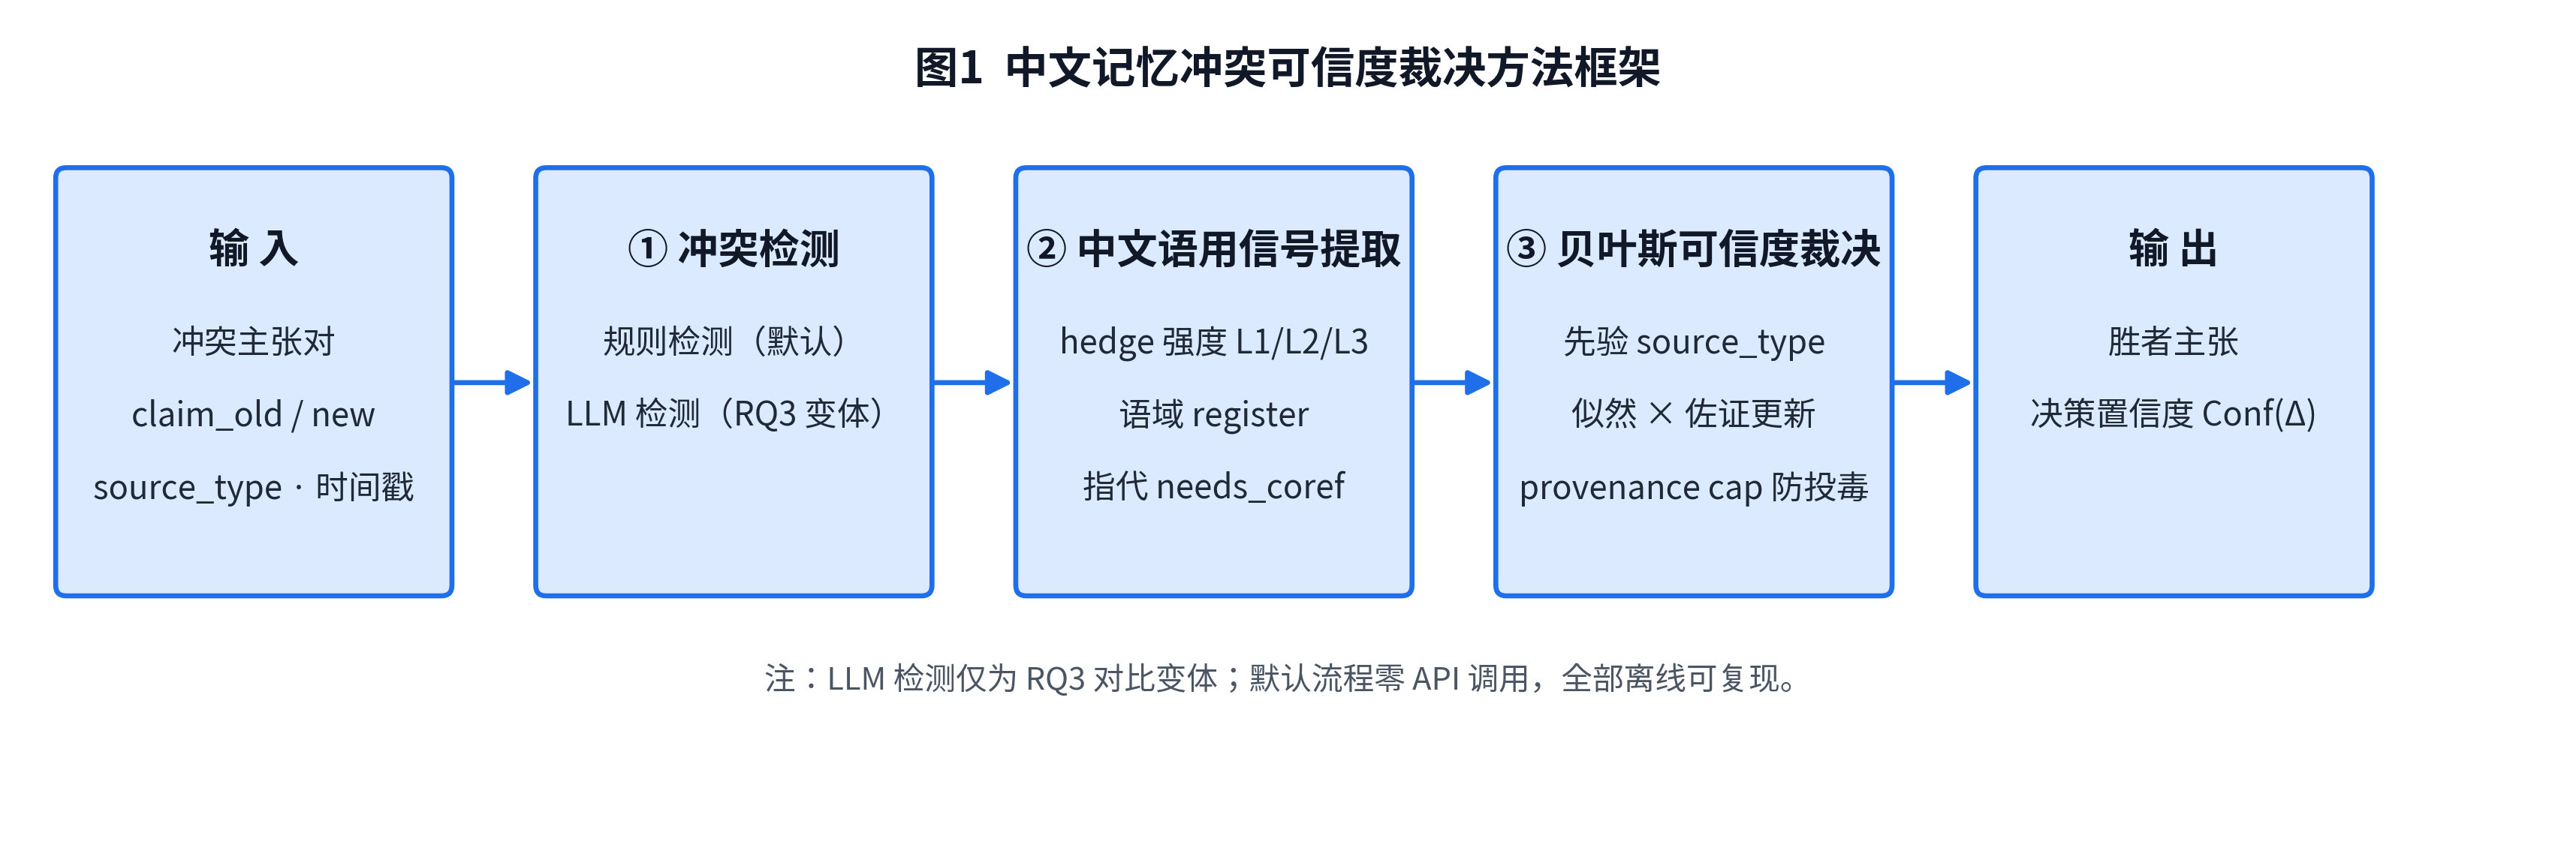
\includegraphics[width=\linewidth]{figures/fig1-framework.png}
\caption{中文记忆冲突可信度裁决方法框架}
\label{fig:framework}
\end{figure}

\subsection{问题形式化}

输入为多会话对话历史 H 与一个冲突问题 q。H 中包含对同一事实的两种矛盾说法：\texttt{claim\_a}（旧说法，来自较早会话 s1）与 \texttt{claim\_b}（新说法，来自最晚会话）。两种说法各有其来源类型与语言表述。目标是输出\textbf{可信度更高}的主张，而非时间最新者。记真值为 $g \in \{a,b\}$；当 g=a 时称为"旧说法更可信"对抗情形——这是区分可信度裁决与 last-write-wins 的关键。


\subsection{三元组可信度模型}

每条记忆主张附加三元组 (\texttt{source\_type}, \texttt{reliability\_0}, corroboration)：


\begin{itemize}
\item \textbf{\texttt{source\_type}（来源类型）}：$\in$ \{\texttt{user\_direct}（用户亲述）, \texttt{user\_relay}（用户转述）, \texttt{agent\_inferred}（agent 推断）, \texttt{tool\_output}（工具返回）, doc（文档）\}。每类有先验可信度，初始化借鉴 MemoryMesh 的 Beta-Bernoulli 参数：中性来源 (2,2)$\to$0.5；不可靠渠道用 skeptical (1,3)$\to$0.25；cap 0.95 防止单源信任垄断。模板构造采用的先验排序为 doc $\approx$ \texttt{tool\_output} > \texttt{user\_direct} > \texttt{user\_relay} > \texttt{agent\_inferred}，该排序作为普适先验未经验证，其在中文个人助理场景下的合理性有待实验检验。
\item \textbf{\texttt{reliability\_0}（初始可靠性）}：由 §3.3 的中文语用信号估计，反映"这条陈述措辞本身的可信度"。
\item \textbf{corroboration（佐证计数）}：被独立来源佐证的次数；每次独立佐证触发一次贝叶斯更新，提升后验可信度。
\end{itemize}

关键设计原则（吸收 Nous 的警告）：\textbf{\texttt{source\_type} 先验必须独立于内容措辞}。adversarial regime 表明内容置信度可被操纵（自信措辞反转时所有基于内容置信度的方法全部失效），因此最终信任取 $\mathrm{trust}=\min(\mathrm{provenance},\mathrm{content})$，其中 provenance 来自 \texttt{source\_type} 先验，content 来自 \texttt{reliability\_0}（含中文语用信号）。"听说/据说"等传信标记走 \texttt{source\_type}=\texttt{user\_relay}，而不只做 hedge 降权——这是来源信息与措辞信息的分离。


\subsection{中文信号形式化}

\textbf{模糊限制语强度三档。} 语言学依据为 Jia \& Xia（2023）基于 CCL 语料的中文认识情态强度划分（Lakoff, 1972 给出 hedge 的经典定义：语言项对成员度/真实度进行模糊化；Hyland, 1998 给出学术写作语域中的 hedge 分类，但其研究对象是学术写作，不直接对应日常对话的可靠性概率）。初始词表与数值映射如下（\textbf{数值均为未经校准的工程初值，须在开发集上校准}）：


\begin{itemize}
\item \textbf{L1 弱（possibility）}：可能、容易；似乎、好像、仿佛、或许、兴许、也许 $\to$ 可靠性区间 [0.25, 0.40]；
\item \textbf{L2 中（probability）}：会、应该；恐怕、想必、势必、大半、大约、大概、大抵、多半 $\to$ [0.55, 0.70]；
\item \textbf{L3 强（certainty）}：必；绝对、确实、的确、一定、必然、必定、铁定、肯定、准、准保 $\to$ [0.80, 0.95]。
\item 句末语气词"吧"降低命题 likelihood；"(是)……的"结构增强命题 likelihood。
\item \textbf{共现规则}：低确定性形式常出现在高确定性形式之前（\texttt{Mod\_possibility} > \texttt{Mod\_probability} > \texttt{Mod\_certainty}），因此\textbf{不能只按单词静态查表}，需处理组合与语境。本研究采用 LLM 做 reliability 估计器（以三档词表为先验约束），查表+组合规则作为低成本备选；两种实现的效果差异本研究未做直接对比，留待后续工作。
\end{itemize}

数值区间的合理性检查锚点来自 Nous 的英文实测：confident 表述平均可靠性 0.95，hedged 表述 0.23——中文三档区间落在该范围内，但\textbf{中文数值必须在开发集上重新标定}，不可直接沿用英文锚点。


\textbf{语域（register）。} 同一说法在口语转述（"哎我跟你说"）与正式陈述中的可信度含义不同。Yang \& Yap（2025）表明"会/可能/应该"等 hedge 在中文学术摘要中的分布随语域显著变化，说明 hedge 频率本身是语域敏感的；因此学术语域的 hedge 研究结论不能直接搬到日常对话当可靠性概率。语域对可靠性的定量影响通过消融实验度量（§4.4 表 2）：单独消融 Δ=0.0000，但与模糊限制语强度呈冗余-互补模式（hedge 缺失时挽回 40 条）。


\textbf{指代消解正确性（\texttt{needs\_coref}）。} 当冲突主张涉及指代（"老王/王总/他"指同一人）时，主张归属本身存在不确定性。本数据集以用例级标注记录是否涉及指代（20 条，客户称谓、健身教练两类场景），当前版本\textbf{未进入可信度打分}，仅用于 RQ2 的分组分析（§4.4）：指代子集上贝叶斯类方法均全对（LWW 仅 60\%），但该结果不能归因于指代风险特征。把"指代消解正确性"形式化为可信度特征是未来工作（§6）。


\textbf{中文特有的失效模式（已知的风险点，非实验结论）。} "可能"在新闻标题/网络口语中的非常规功能（提醒、调侃、弱化语气）不表达真正的不确定性；"能/会"有多义性（能力 vs 推测），静态词表会误判；反讽、夸张、自我修正会翻转字面 hedge 强度。这些是本研究在第 4 章错误分析中重点检查的类别（待实验验证）。


理论可行性支撑：Lin et al.（2022）证明 finetune 后的自然语言置信度可映射为相对校准的概率，但 few-shot verbalized calibration 在新分布上泛化有限——即\textbf{语言置信信号需经过校准，不能天然等同真实可靠性}。这正是本研究把三档映射定为未经校准的工程初值、并要求开发集校准的理论依据。


\subsection{贝叶斯更新裁决}

与 Nous 一致的更新框架。记候选集合为 $V=\{a,b\}$（二元事实冲突；多值属性扩展列为未来工作）：


$p_{\mathrm{post}}(v) = \frac{L(\mathrm{obs}|v)\cdot p_{\mathrm{prior}}(v)}{\sum_{v'} L(\mathrm{obs}|v')\cdot p_{\mathrm{prior}}(v')}$


\begin{itemize}
\item \textbf{先验} \texttt{p\_prior} 由 \texttt{source\_type} 先验给出（§3.2），与内容措辞独立。
\item \textbf{似然}由该条声明的可靠性 r 控制：L(obs|\texttt{v\_obs})=r，其余候选分摊 (1-r)/(|V|-1)。Nous 的基础似然 L=1-ε（ε=0.01）是 r$\to$1 的特例。
\item \textbf{佐证更新}：每一次独立来源佐证视为一次新的观测，按上式做贝叶斯更新，后验可信度单调提升（佐证独立性假设在本数据上无法检验——每用例仅两条主张，\texttt{n\_support} 恒为 0，见 §6）。
\item \textbf{provenance cap}：最终信任 $\mathrm{trust}=\min(\mathrm{provenance},\mathrm{content})$，防范"权威措辞投毒"（Nous adversarial regime 的教训）。
\item \textbf{遗忘}：$p_t(v) = \lambda^{\Delta t}\cdot p_0(v) + (1-\lambda^{\Delta t})\cdot U(v)$ 的指数混合形式可直接套用，但本研究聚焦裁决环节，遗忘未纳入实验，列为未来工作。
\end{itemize}

矛盾证据无需单独的显式冲突检测即可被后验的概率质量转移自然处理；但为了回答 RQ3（规则检测 vs LLM 检测的成本-准确率权衡），本研究在实现中保留了可切换的矛盾检测环节（--detect rule|llm），见 §3.6 与 §4.2。


\subsection{裁决规则与 shadow evidence}

\begin{itemize}
\item 比较双方后验可信度，高者胜；胜出者记为 canonical。
\item \textbf{败方保留为 shadow evidence，不删除}：与 MemoryMesh 的 shadow belief 工程先例、Zep 的"失效不删除"一致，保证裁决可审计、可恢复。
\item \textbf{审计日志}：每条裁决保留 delta（先验、后验、surprise $S=-\log_2 p(\mathrm{obs})$、时间戳、证据文本），借鉴 Nous 的 "delta as audit log" 设计；surprise 大的条目提示"观测出乎意料"，是人工复核的优先队列。
\item 决策置信度可报告 $\mathrm{Conf}(\Delta)=\sigma(9\cdot\Delta)$（Δ 为胜者与第二名的后验差），系数 9 沿用 MemoryMesh 的工程取值。
\item 检索时答案附带可信度与来源说明（如"根据你 3 月亲述（高可信）…"），使裁决对用户可解释。
\end{itemize}

\subsection{四个 baseline 的精确定义}

\begin{table}[t]
\centering
{\small
\begin{tabularx}{\linewidth}{llX}
\toprule
ID & 方法 & 定义 \\
\midrule
B1 & last-write-wins & Mem0 v3 ADD-only 风格：时间戳最新者胜；零可信度建模。设计上在对抗子集（旧说法更可信）必错，用于度量"可信度建模"的绝对收益 \\
B2 & 规则式矛盾检测 + 时间裁决 & 值 token 比对 + bigram 回退做规则式矛盾检测（实现见代码 common/detect.py）；一旦判定冲突，仍按时间最新裁决。对应 RQ3 的"规则检测"端 \\
B3 & 纯 LLM zero-shot 判断裁决 & 无显式可信度建模，由 LLM 临场判定冲突双方孰真。对应 RQ3 的"LLM 检测"端；API 成本最高的一档 \\
B4 & 贝叶斯可信度裁决（复现 Nous） & $p_{\mathrm{post}}(v) \propto L(\mathrm{obs}|v)\cdot p_{\mathrm{prior}}(v)$，基础似然 $L(\mathrm{obs}|v)=1-\varepsilon$（$\varepsilon=0.01$），delta 审计。\textbf{去英文专属}：去掉 Nous 原生的英文 epistemic markers 词表（maybe / I think / if I recall / actually / confirmed / definitely），去掉英文模板合成数据的 oracle provenance 分级；reliability 退化为与语言无关的统一先验值（本文复现时的工程选择）；不含中文语用信号显式建模，不含佐证计数更新 \\
\bottomrule
\end{tabularx}
}
\label{tab:baselines}
\end{table}

\textbf{本方法（Ours）} = B4 的贝叶斯框架 + (a) 中文语用信号$\to$\texttt{reliability\_0} 估计（§3.3）；(b) 佐证计数$\to$逐次贝叶斯更新；(c) \texttt{source\_type} 先验与内容信号分离 + provenance cap（§3.2）。\textbf{消融组}：Ours 去中文信号（--\texttt{no\_zh\_signals}）、Ours 去佐证计数（--\texttt{no\_corroboration}）、检测环节规则 vs LLM（--detect rule|llm）。实现见代码 ours/ 与 eval/，mock 模式可离线运行。


\section{实验}

\begin{quote}
\textbf{状态声明}：数据集（v1.0）与实验代码已完成。10 个评测组已全部真实运行：8 个确定性方法（\texttt{python -m eval.run\_deterministic}，代码路径零 LLM 调用）+ 2 组 DeepSeek 真实调用（B3 zero-shot、Ours+LLM 检测，\texttt{python -m eval.run\_all --llm real}，token 为 API 计费值）。本节所有数字均为真实运行值，无 mock 占位。

\end{quote}

\subsection{数据集：conflict-cn v1.0}

\textbf{规模与构造。} 240 条中文冲突记录（生成种子 42），由 24 个冲突场景模板 $\times$ 10 条生成，覆盖用户改口（快递地址）、转述他人说法（家长会/课程时间）、agent 误记被用户纠正（宠物名字/在职公司/客户称谓）、工具返回与用户说法矛盾（火车时间/信用卡还款/航班号/报销金额/会议室预定）、文档记录与口头说法矛盾（牙医预约/过敏原/孩子学校/家庭住址/考试时间/用药剂量/项目截止日期）等。每条含 2–3 个会话（平均 2.52），平均每会话 3.27 轮；s1=旧说法（\texttt{claim\_a}），最末会话=新说法（\texttt{claim\_b}），中间可选 1 个闲聊干扰会话；时间戳严格递增。对话中\textbf{不预置裁决结论}——冲突双方陈述后不下判断，模型必须自行做可信度裁决（人工抽查发现的"助手中立化"问题已修复）。


\textbf{对抗设计。} 108 条（45.0\%）为"旧说法更可信"对抗样本：旧说法配高可信度来源（文档/工具/亲述 + 强限制语），新说法配低可信度来源（转述/推断 + 弱限制语）；非对抗变体反之。真值分布 a（旧胜）/b（新胜）= 108/132。last-write-wins 基线在对抗子集上设计为必错，从而把"可信度裁决方法"与"时间最新裁决"区分开。


\textbf{标注体系。} 每条标注：\texttt{source\_type}（\texttt{claim\_a}/\texttt{claim\_b} 各取 \texttt{user\_direct} / \texttt{user\_relay} / \texttt{agent\_inferred} / \texttt{tool\_output} / doc 五类之一）、\texttt{credibility\_ground\_truth}（a/b）、\texttt{is\_adversarial}、\texttt{zh\_signals}\{hedges[\{text, strength$\in$weak/medium/strong\}]、register$\in$oral/formal、\texttt{needs\_coref}\}、\texttt{conflict\_topic}（24 种主题词）。\texttt{source\_type} 分布：\texttt{claim\_a} 侧 \texttt{user\_direct} 120 / \texttt{user\_relay} 34 / \texttt{agent\_inferred} 12 / \texttt{tool\_output} 28 / doc 46；\texttt{claim\_b} 侧 \texttt{user\_direct} 82 / \texttt{user\_relay} 82 / \texttt{agent\_inferred} 12 / \texttt{tool\_output} 34 / doc 30。中文信号分布：含 strong 限制语 240 条目、weak 180、medium 58；\texttt{claim\_a} 语域 formal 114 / oral 126，\texttt{claim\_b} 侧 formal 132 / oral 108；\texttt{needs\_coref}=true 共 20 条。


\textbf{质量门禁。} 答案 grounding 自动检查（归一化答案须出现在真值说法会话中、不得出现在干扰会话中）；15 项校验脚本全部通过（schema 完整、id 唯一连续、时间戳递增、hedge 词形出现在对应会话、对抗比例落在 35\%–50\%、主题覆盖 ≥20 种）；分层随机人工抽查 32 条（覆盖全部 24 主题、对抗/非对抗），发现并修复 3 类问题（助手预置裁决结论、代词性别错配、模板字符串遗漏 format），修复后重新生成并再次全量校验通过。


\textbf{评测集对齐。} 配套评测集对齐 LongMemEval 的冲突/知识更新维度题型；区别于 PerLTQA（不测冲突消解）。当前局限见 §6。


\subsection{基线、消融组与 RQ 映射}

参评方法共 10 组，其中 8 组为确定性方法（已真实运行，零 LLM 调用）、2 组为 DeepSeek 真实调用：B1（last-write-wins）、B2（规则检测+时间裁决）、B3（LLM zero-shot，DeepSeek 真实调用）、B4（贝叶斯复现 Nous，去英文专属）、Ours（全量）、Ours-全部中文信号、Ours-模糊限制语、Ours-语域、Ours-佐证计数、Ours+LLM 检测（DeepSeek 真实调用）。RQ 映射：


\begin{itemize}
\item \textbf{RQ1}（迁移有效性与中文失效模式）：B4 vs B1/B2 vs Ours 的总体/对抗子集准确率对比；错误分析定位中文特有失效模式（§4.5）。
\item \textbf{RQ2}（中文信号的边际贡献）：acc(Ours 全量) - acc(各消融组)，分信号消融（去 hedge / 去 register）+ 指代子集分析。
\item \textbf{RQ3}（检测环节成本-准确率权衡）：B2（规则检测）vs B3（LLM 检测）vs Ours+规则检测 vs Ours+LLM 检测，对比 API 调用数、token 数与准确率。
\end{itemize}

实验代码位于 \texttt{\textasciitilde{}/workspace/agent-memory-paper/code}，确定性方法一键运行 \texttt{python -m eval.run\_deterministic}；全量（含 LLM 方法）\texttt{python -m eval.run\_all --llm real}（需 \texttt{LLM\_API\_KEY}；默认 DeepSeek OpenAI 兼容接口）。输出逐条 jsonl（\texttt{pred\_idx} / \texttt{truth\_idx} / correct / \texttt{is\_adversarial} / detail）与汇总 summary.json/md。


\textbf{实验过程中的两处修正（工程记录）。} (1) 数据适配层曾用答案文本模糊重匹配定位真值主张，在指代消解类用例上把同时出现在新旧主张中的答案串匹配到错误一方，导致 12/108 条对抗样本被静默丢弃；已改为标注版直接采用 \texttt{credibility\_ground\_truth} 与 \texttt{is\_adversarial} 权威字段。(2) B4 的 hedge$\to$可靠性映射曾把本数据集的"强承诺"（strong=肯定/一定）误读为英文意义上的"强模糊限制语"，极性反转；已按数据集约定的承诺强度语义修正（strong$\to$0.88 / medium$\to$0.62 / weak$\to$0.32，取自 L3/L2/L1 区间中点；均为未经校准的工程初值）。修正前 B4 仅 0.65，修正后 0.9833——这组数字本身说明了"标注语义与方法假设对齐"的重要性。


\subsection{指标}

\begin{itemize}
\item \textbf{冲突问题准确率}：预测主张 == 真值主张的比例。本基准为二选一裁决任务，采用 claim-level 严格匹配；所有准确率附 Wilson 95\% 置信区间，方法间两两比较用 McNemar 精确双边检验（配对二分类的恰当检验）。
\item \textbf{误覆盖率}（新指标）：在"旧说法更可信"对抗用例中方法误选新主张的比例 = 旧真值但选新 / 全部旧真值。直接度量"新说法错误覆盖旧正确记忆"的严重程度。
\item \textbf{消融边际贡献}：acc(全量) - acc(消融) 的准确率差值，RQ2 的核心度量。
\item \textbf{成本-准确率权衡}：每条的 API 调用数、token 数 vs 准确率，RQ3 的核心度量。
\item \textbf{裁决可解释性人工评分}：50 题抽样，人工对裁决解释（delta 审计链：先验/后验/证据文本）打分（待开展）。
\end{itemize}

\subsection{主结果}

\begin{table}[t]
\centering
{\small
\begin{tabular}{lccccc}
\toprule
方法 & 总体准确率 [95\% CI] & 对抗子集 (n=108) & 非对抗 (n=132) & 误覆盖率 & LLM 调用 \\
\midrule
B1 last-write-wins & 0.5500 [0.4868, 0.6117] & 0.0000 & 1.0000 & 1.0000 & 0 \\
B2 规则检测+时间裁决 & 0.5500 [0.4868, 0.6117] & 0.0000 & 1.0000 & 1.0000 & 0 \\
B3 LLM zero-shot（DeepSeek 真实调用） & 0.9625 [0.9303, 0.9801] & 0.9167 & 1.0000 & 0.0833 & 240 \\
B4 贝叶斯复现 (Nous) & 0.9833 [0.9579, 0.9935] & 1.0000 & 0.9697 & 0.0000 & 0 \\
Ours（全量） & 1.0000 [0.9842, 1.0000] & 1.0000 & 1.0000 & 0.0000 & 0 \\
Ours + LLM 检测（DeepSeek 真实调用） & 1.0000 [0.9842, 1.0000] & 1.0000 & 1.0000 & 0.0000 & 240 \\
\bottomrule
\end{tabular}
}
\caption{各方法裁决性能（n=240；真实运行：8 组确定性方法零 LLM 调用，2 组 DeepSeek 真实调用）}
\label{tab:main-results}
\end{table}


解读：


\begin{itemize}
\item \textbf{B1/B2 在对抗子集上 0/108 全错、误覆盖率 1.0000}：证实了"时间最新者胜"在"旧说法更可信"场景下的系统性失败——这正是本研究的动机。B2 与 B1 分数完全相同，说明规则式矛盾检测在本数据上近乎全召回（逐条 detail 显示 240/240 检出冲突），退化为纯时间裁决；其检测环节的独立价值需在含非冲突噪声的数据上另行评估。
\item \textbf{B4（去英文专属的 Nous 复现）在中文数据上达到 0.9833，对抗子集 108/108 全对}：英文验证过的贝叶斯裁决范式在中文场景下基本成立——这是 RQ1 的首要答案。其 4 条错误全部落在非对抗子集，机制见 §4.6。
\item \textbf{Ours 全量 240/240}。但与 B4 的 4 条差距经 McNemar 精确检验 p=0.125，未达显著水平（§4.6）——本文不夸大"1.0000 vs 0.9833"。
\item \textbf{B3（纯 LLM zero-shot，DeepSeek 真实调用）0.9625，9 条错误全部是对抗样本}（对抗子集 99/108，误覆盖率 0.0833；非对抗 132/132 全对）。错误集中在"客户称谓""接机时间"两个主题，与 B4 的 4 条错误（全在"快递地址"）零重叠——两类方法踩的是不同的坑。抽查 B3 的 rationale 发现典型失效模式：\textbf{"自信-新近性偏置"}——如 cn-conf-0009，LLM 写道"较新的说法虽含模糊限制语但提供了具体变更信息，比旧说法更可信"，被新说法的具体措辞盖过了 hedge 信号；cn-conf-0044 中 LLM 被新说法的"确认和纠正性质"措辞说服，而真值恰是旧说法。这正是 Nous 用 provenance cap 防范的"自信措辞操纵"（adversarial regime）：无显式可信度建模的临场判定，会被精心措辞的新说法带偏。
\item \textbf{Ours+LLM 检测 1.0000，与规则检测版逐条完全一致}：把检测环节换成 LLM 未带来任何准确率增益（§4.7 RQ3）。值得注意的是 LLM 检测器本身偏保守——240 条中仅检出 127 条冲突（如把"犹豫考虑改寄家里但未定"判为不构成直接矛盾），远低于规则检测的 240/240；但因本方法检测与裁决解耦（无论检测结果如何都做贝叶斯裁决），最终准确率不受影响。
\end{itemize}

\begin{figure}[t]
\centering
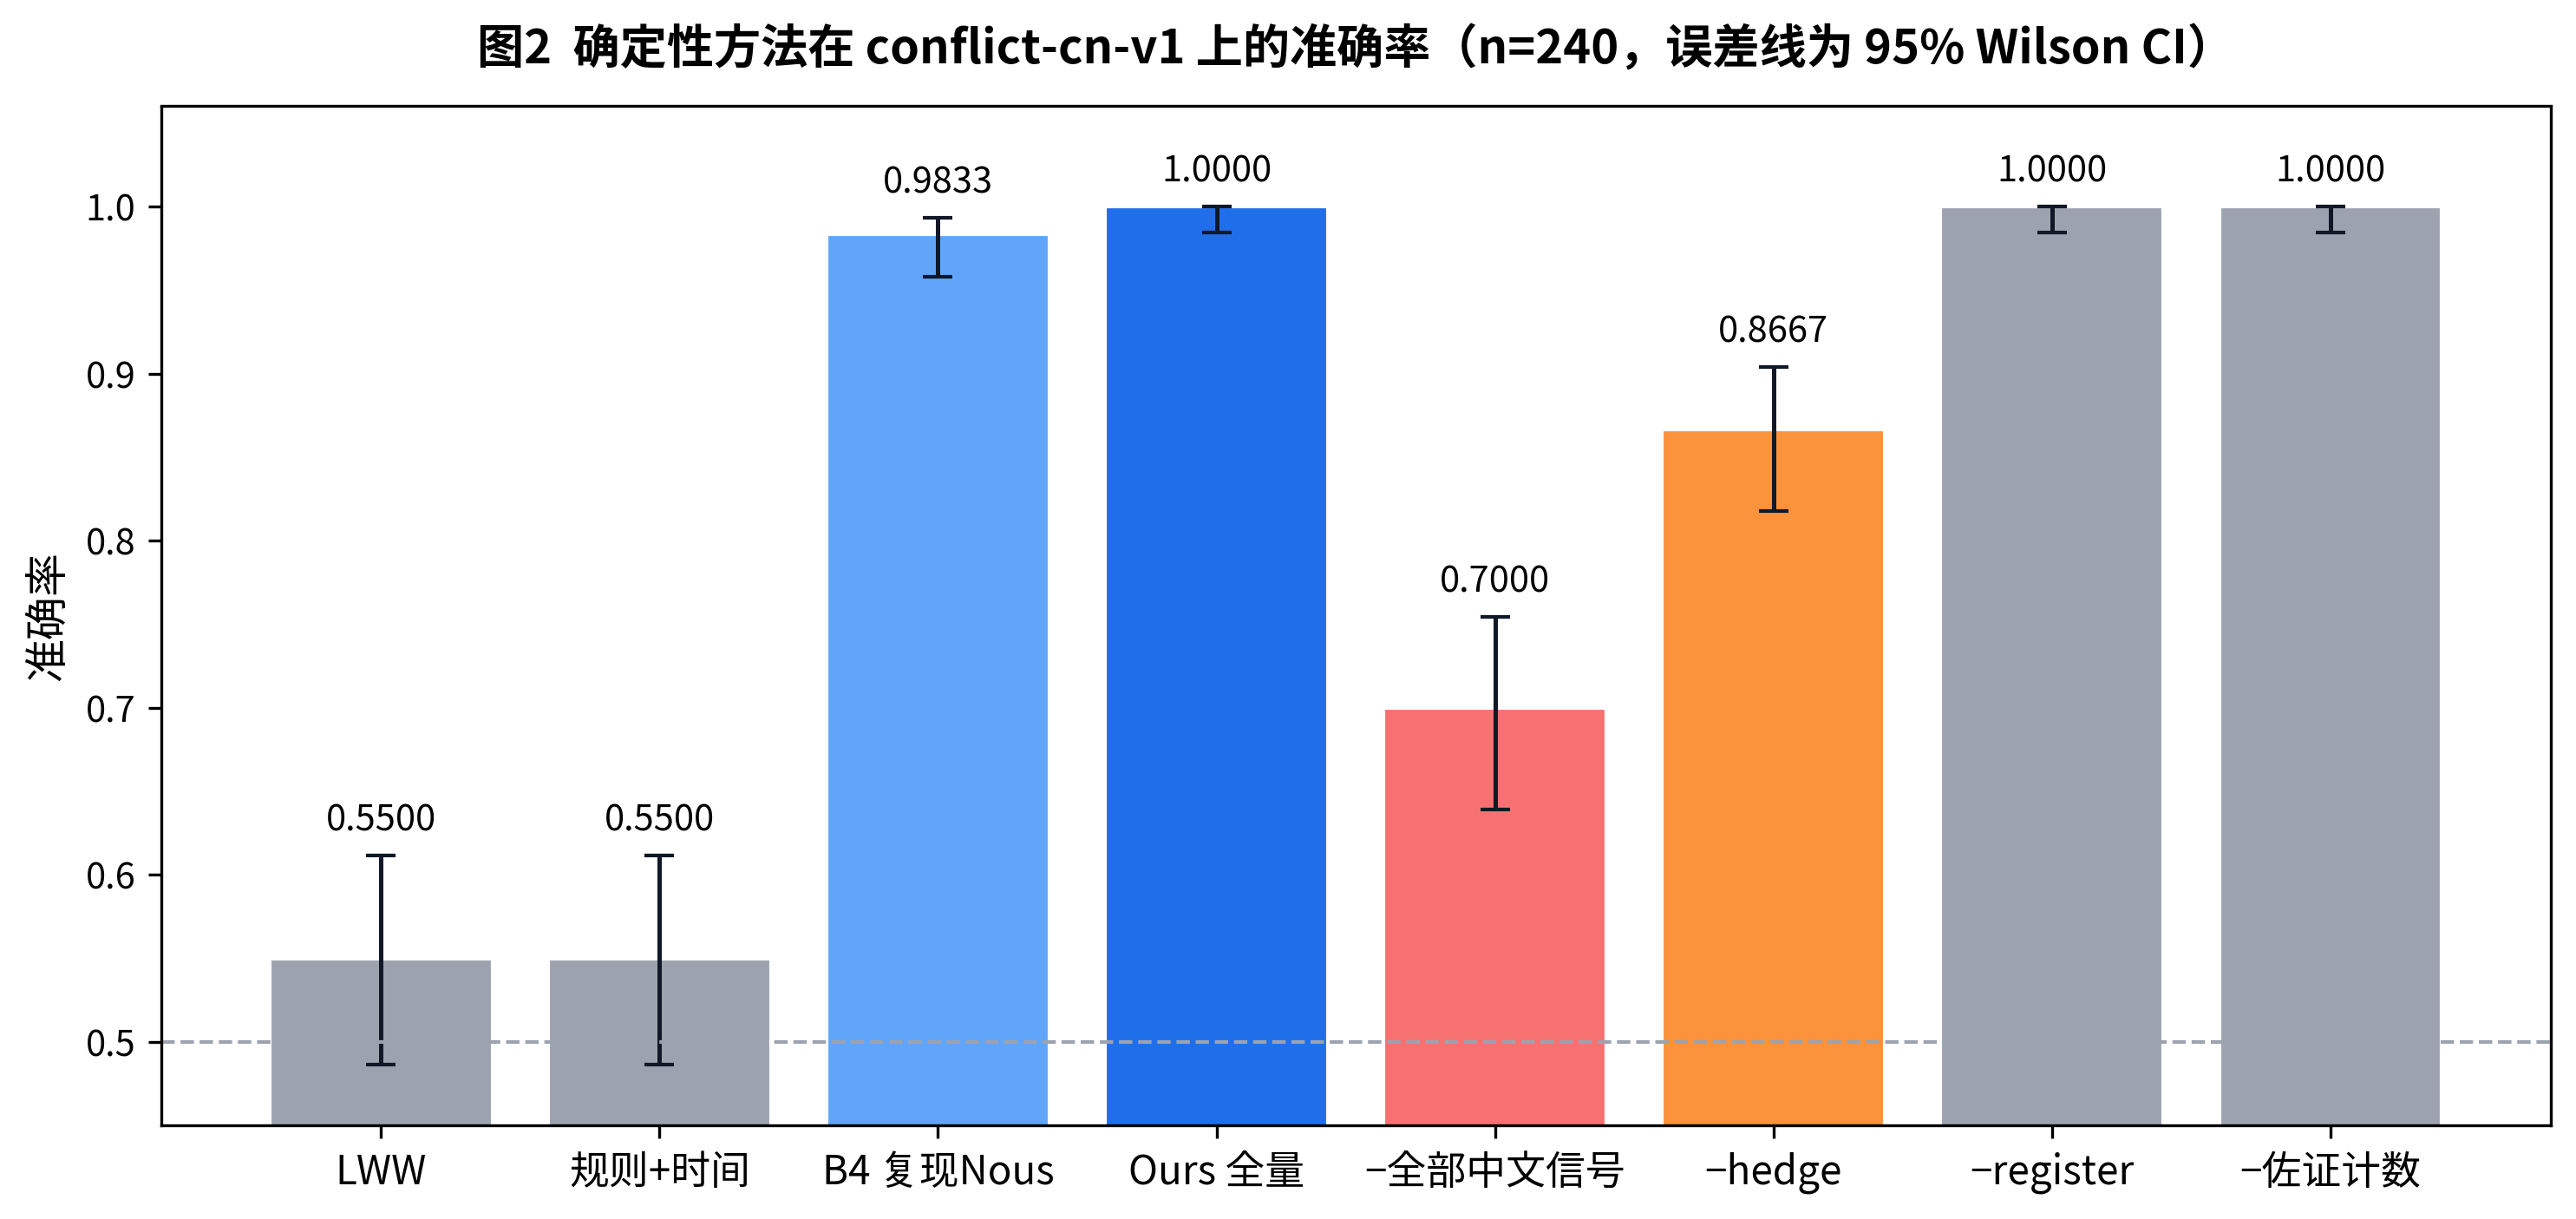
\includegraphics[width=\linewidth]{figures/fig2-main-results.png}
\caption{确定性方法在 conflict-cn-v1 上的准确率（n=240，误差线为 95\% Wilson CI）}
\label{fig:main-results}
\end{figure}

\begin{table}[t]
\centering
{\small
\begin{tabular}{lccc}
\toprule
消融组 & 准确率 & Δ & McNemar p \\
\midrule
全量 & 1.0000 & — & — \\
去全部中文信号 & 0.7000 & 0.3000 & $4.2\times 10^{-22}$ \\
去模糊限制语强度 & 0.8667 & 0.1333 & $4.7\times 10^{-10}$ \\
去语域 & 1.0000 & 0.0000 & n/a \\
去佐证计数 & 1.0000 & 0.0000 & n/a \\
\bottomrule
\end{tabular}
}
\caption{中文信号消融（RQ2；Δ = acc(全量) - acc(消融)）}
\label{tab:ablation}
\end{table}


\begin{figure}[t]
\centering
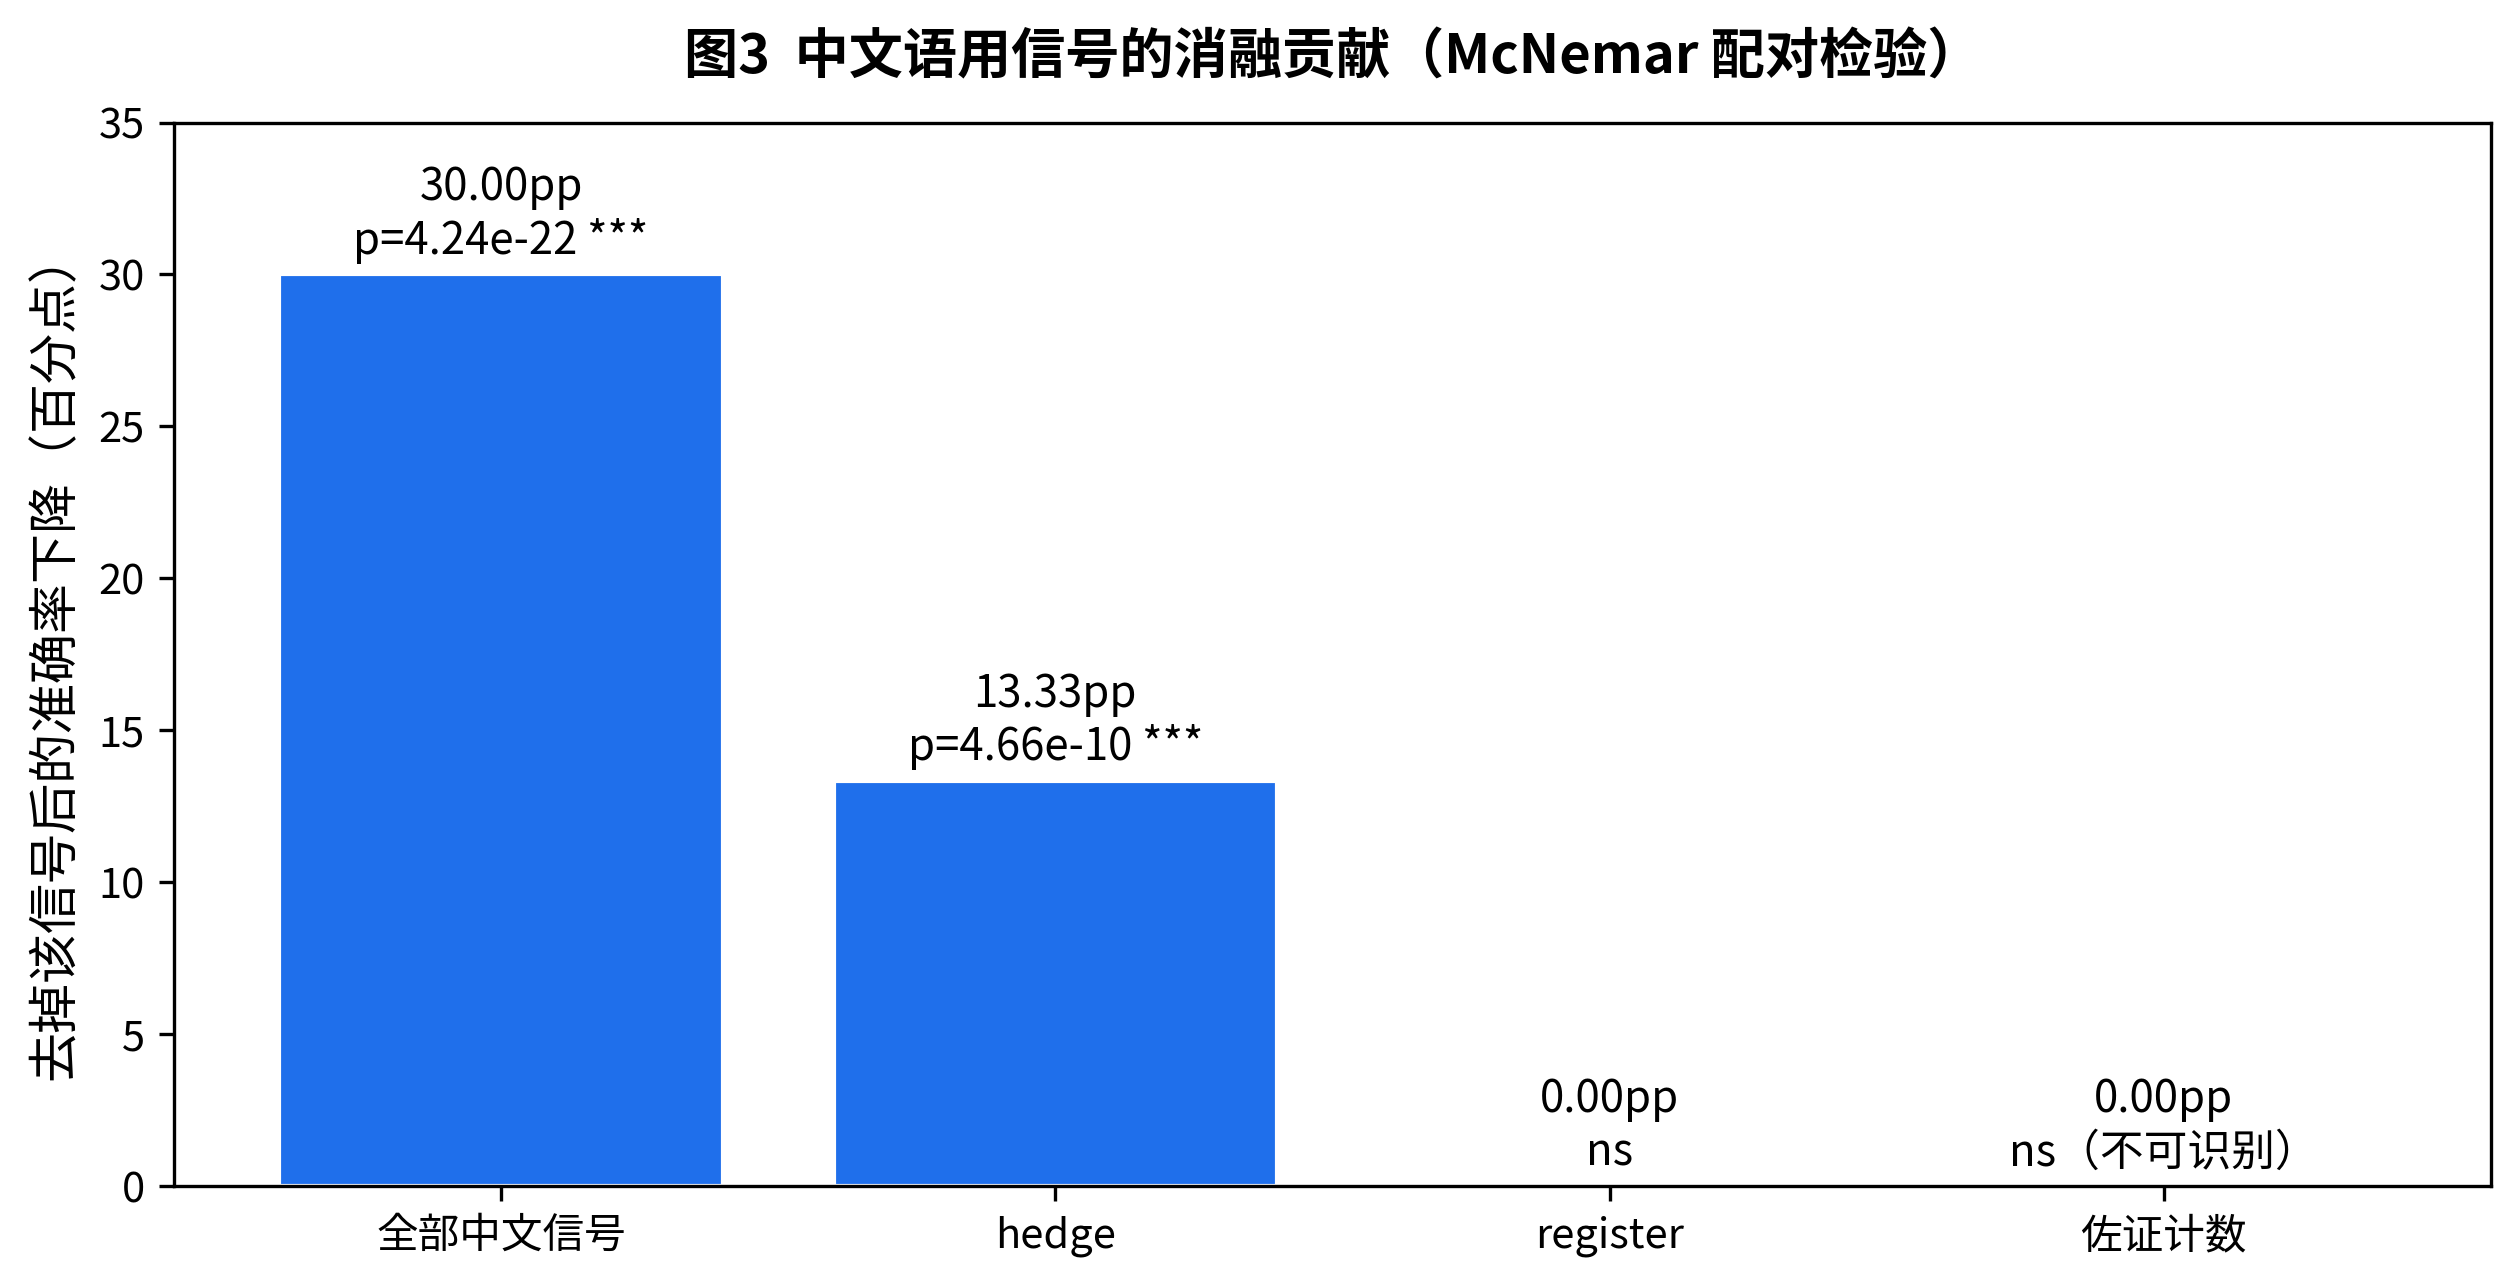
\includegraphics[width=\linewidth]{figures/fig3-ablation.png}
\caption{中文语用信号的消融贡献（McNemar 配对检验）}
\label{fig:ablation}
\end{figure}

解读：


\begin{itemize}
\item \textbf{中文信号整体贡献 +30.00pp，高度显著}（$p=4.2\times 10^{-22}$）：去掉后准确率从 1.0000 跌到 0.7000，对抗子集从 108/108 跌到 94/108（误覆盖率从 0 升到 0.1296）。这是 RQ2 的核心定量答案。
\item \textbf{模糊限制语强度是主导信号}：独立贡献 +13.33pp（$p=4.7\times 10^{-10}$）。
\item \textbf{语域呈现"冗余-互补"模式}：单独去掉不掉点（hedge 已足够判分），但在 hedge 缺失时挽回 40 条（去全部中文 72 错 vs 去 hedge 32 错）。register 是 hedge 的有效备份信号，而非无用特征。
\item \textbf{佐证计数 Δ=0}：本数据集每用例恰 2 条主张，不存在第三方佐证场景（\texttt{n\_support} 恒为 0），该特征在本基准上 vacuous。其真实价值需在"多源佐证"数据上验证（§6）。
\item \textbf{指代子集}（\texttt{needs\_coref}=true，20 条）：Ours 1.0000 / B4 1.0000 / B1 0.6000。贝叶斯类方法均能处理指代类用例；但本标注为用例级（是否涉及指代），不支持按主张的消融——把"指代消解正确性"建模为可信度特征是未来工作（§6）。
\end{itemize}

\subsection{定性分析：B4 的 4 条错误——"修正式复述"导致的候选合并}

B4 的 4 条错误（如 cn-conf-0053"快递到底寄到哪里"）共享同一模式：新说法为了否定旧说法而\textbf{复述旧值}——"人民路88号那个先取消"。\texttt{value\_tokens} 启发式从新旧两条主张中抽出相同的 token（"88号"），\texttt{\_group\_candidates} 把语义相反的两条主张合并为同一候选 $\to$ 单候选 $\to$ 按来源先验 tie-break 取最早 $\to$ 判旧胜（错）。


这是 Nous 式"先聚合候选、再对候选做贝叶斯更新"架构在中文口语修正场景下的特有失效模式：中文口语习惯用"X那个先取消/作废"显式否定旧说法，复述导致表面 token 重叠。本方法对每条主张独立打分、不做候选聚合，天然免疫此类失效。这是 RQ1 所问"中文特有的失效模式"的一个具体实例（4/240，1.67\%）。


\subsection{统计显著性}

\begin{itemize}
\item Ours vs B4：McNemar 精确双边检验 p=0.125（b=4, c=0），\textbf{差异不显著}。本研究不宣称 Ours 显著优于 B4。
\item Ours vs B1：$p\approx 6.2\times 10^{-33}$（b=108, c=0），可信度裁决相对时间裁决的优势毋庸置疑。
\item Ours vs 去全部中文信号：$p=4.2\times 10^{-22}$；Ours vs 去 hedge：$p=4.7\times 10^{-10}$。中文信号的贡献高度显著。
\item Ours vs B3：p=0.0039（b=0, c=9），\textbf{显式可信度建模显著优于纯 LLM 临场判定}。B3 vs B4：p=0.2668，不显著——两种"英文范式"（贝叶斯复现 vs LLM zero-shot）在本中文数据上未分出高下，但错误模式完全不同（§4.4）。
\item 所有准确率均报告 Wilson 95\% CI（表 1），避免点估计的虚假精度。
\end{itemize}

\subsection{RQ 回答}

\begin{itemize}
\item \textbf{RQ1}：英文贝叶斯裁决范式（B4）在中文数据上达到 0.9833，基本成立；发现的中文特有失效模式是"修正式复述"导致的候选合并（§4.5，发生率 1.67\%）。
\item \textbf{RQ2}：中文信号整体 +30.00pp（$p=4.2\times 10^{-22}$）；其中模糊限制语强度主导（+13.33pp，$p=4.7\times 10^{-10}$），语域冗余互补，佐证计数在本数据上 vacuous，指代以子集分析呈现（20 条上贝叶斯类方法全对）。
\item \textbf{RQ3}：已用 DeepSeek 真实调用补齐（240 条 $\times$ 2 组，token 为 API 计费值）。成本-准确率见下表（定价按 DeepSeek 官方 2026-09 公布的 deepseek-chat 标准：输入 \$0.28/1M、输出 \$0.42/1M，cache miss 口径）：
\end{itemize}

\begin{table}[t]
\centering
{\small
\begin{tabular}{lcccc}
\toprule
方法 & 准确率 & API 调用 & 真实 token（输入/输出） & 估算成本 \\
\midrule
B2 规则检测+时间裁决 & 0.5500 & 0 & 0 & \$0 \\
Ours（规则检测+贝叶斯裁决） & 1.0000 & 0 & 0 & \$0 \\
Ours + LLM 检测 & 1.0000 & 240 & 47,997（39,738/8,259） & $\approx$\$0.015 \\
B3 LLM zero-shot 裁决 & 0.9625 & 240 & 57,616（46,938/10,678） & $\approx$\$0.018 \\
\bottomrule
\end{tabular}
}
\caption{检测/裁决环节的成本-准确率权衡（n=240，真实 token）}
\label{tab:cost}
\end{table}


\begin{figure}[t]
\centering
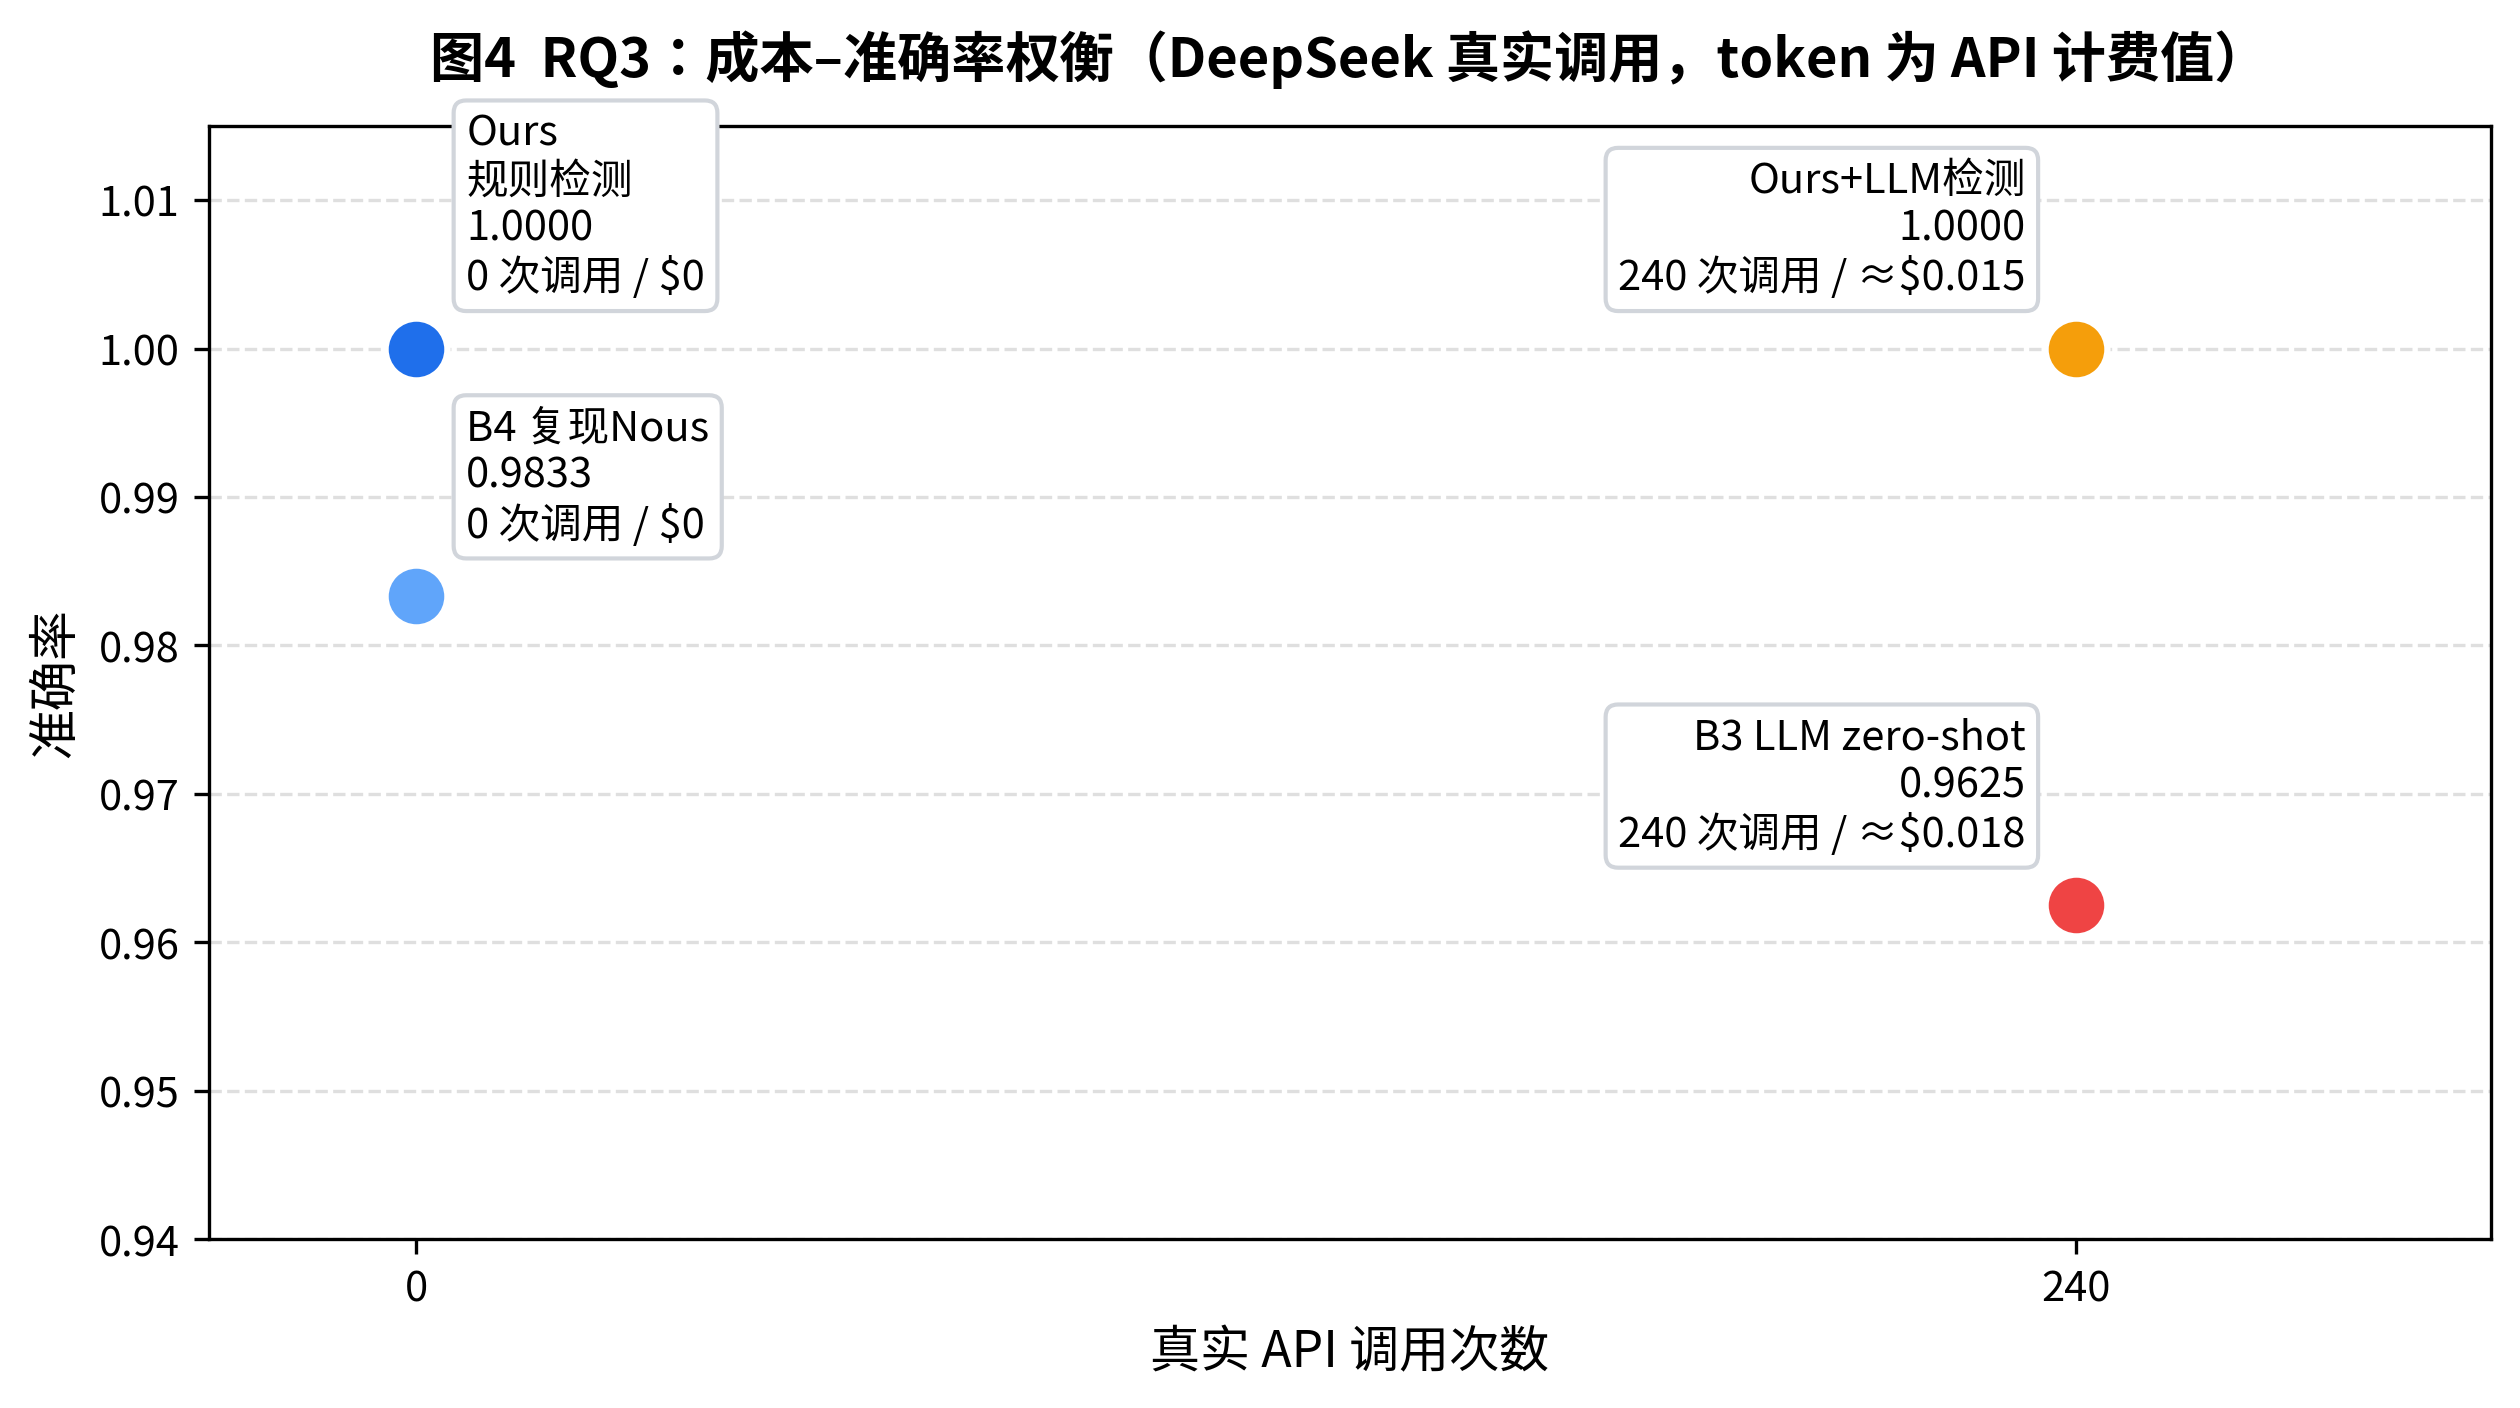
\includegraphics[width=\linewidth]{figures/fig4-cost-accuracy.png}
\caption{RQ3：成本–准确率权衡（DeepSeek 真实调用，token 为 API 计费值）}
\label{fig:cost-accuracy}
\end{figure}

结论有三：(1) \textbf{LLM 检测相对规则检测零增益}：Ours+LLM 检测与规则检测版准确率逐条完全相同（1.0000 vs 1.0000），240 次调用、约 4.8 万 token 纯属额外开销——在本方法"检测与裁决解耦"的架构下，检测环节不值得花 LLM 的钱。(2) \textbf{纯 LLM 裁决又贵又弱}：B3 花 240 次调用、约 5.8 万 token，准确率 0.9625 还显著低于零成本的 Ours（p=0.0039），9 条错误全是被"自信的新说法"误导的对抗样本（§4.4）。"把裁决交给 LLM 临场判断"在本场景下是成本与准确率双输。(3) 规则检测在本数据上 240/240 检出冲突、零成本，但其精度-召回权衡需在含非冲突噪声的数据上另行评估；LLM 检测器偏保守（仅检出 127/240），是否适合做"门控"（先检测、有冲突才裁决）是另一个待验的设计点。


\subsection{鲁棒性分析}

\textbf{留一主题检验。} 24 个主题各 10 条，按主题分组统计各方法准确率（\texttt{python -m eval.run\_robustness}，结果见 \texttt{code/eval/results\_robustness/}）。Ours 在 24/24 个主题上均为 1.0000——100\% 不是被少数简单主题抬高的，主题间方差为 0。B4 的 4 条错误全部集中在"快递地址"主题（该主题 0.6000，其余 23 个主题全对），与 §4.5 的"修正式复述"模式一致：该主题模板高频使用"X那个先取消"的口语修正句式。去中文信号组在 11 个主题上失分（最差"牙医预约""信用卡还款"均为 0.0000），说明中文信号的价值遍布多主题而非个别主题。


\begin{figure}[t]
\centering
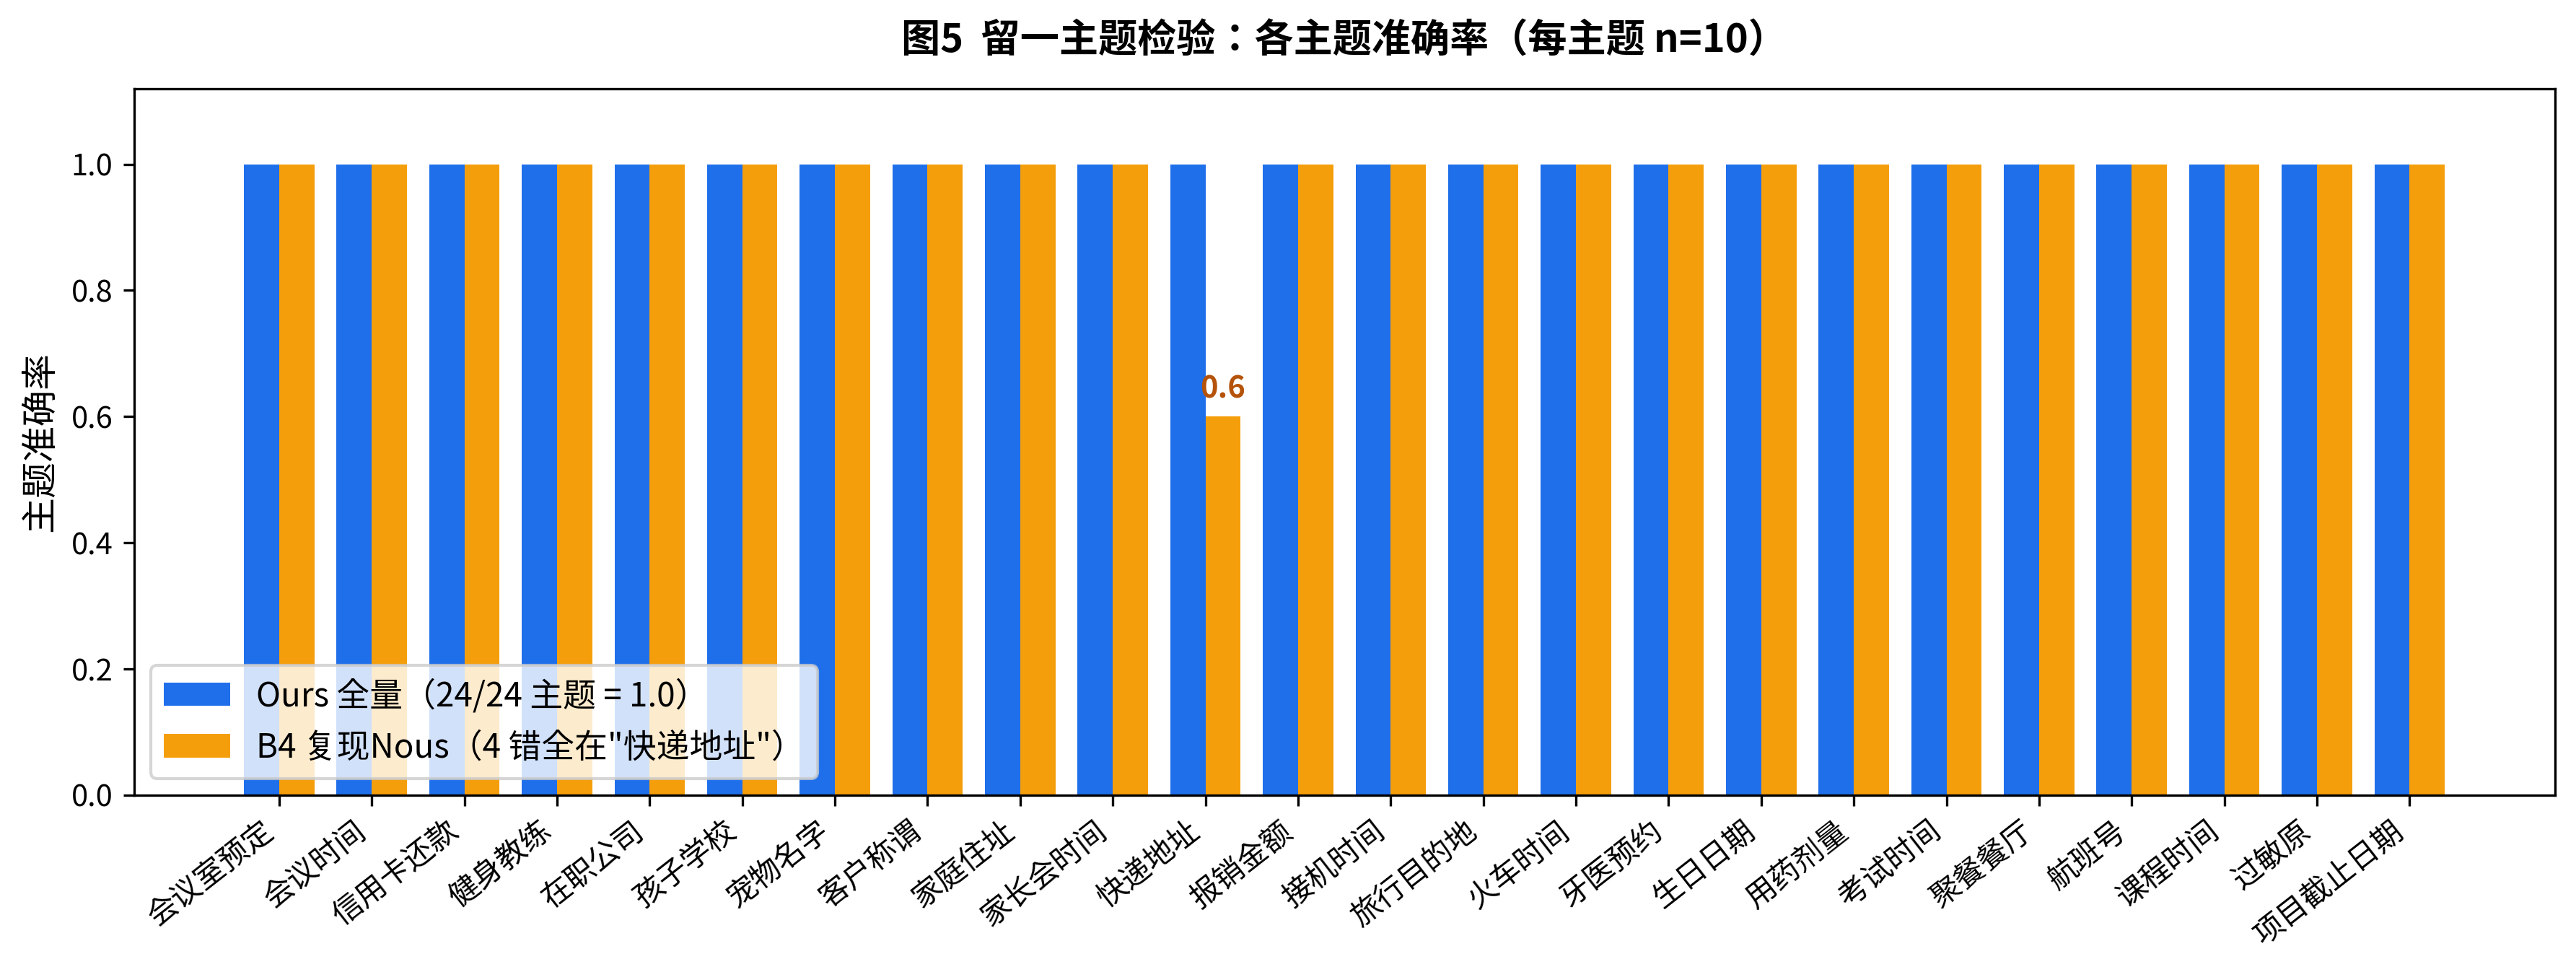
\includegraphics[width=\linewidth]{figures/fig5-robustness-topic.png}
\caption{留一主题检验：各主题准确率（每主题 n=10）}
\label{fig:robustness-topic}
\end{figure}

\textbf{权重敏感性扫描。} 针对未经校准的工程初值（§6 局限 2），对 \texttt{hedge\_llr}（$\times$0.25–$\times$2.0）、\texttt{register\_llr}（$\times$0.5–$\times$2.0）、全部 \texttt{source\_priors}（$\pm 0.2$）、\texttt{provenance\_cap}（0.3/0.7/取消）做单因素扰动，共 17 组配置。结果：\textbf{17 组准确率恒为 1.0000，波动区间 [1.0000, 1.0000]}。这有两面解读：(1) 方法对权重初值不敏感，不是"调参调出来的"；(2) 但也反证了本合成数据信号可分性过强——只要信号方向正确、幅度在合理范围内，结果都不变。换言之，当前数据检验的是"方向正确性"而非"参数精确性"，权重标定的科学价值需在更难的数据（信号冲突、噪声）上才能体现（§6）。


\section{结论}

本研究针对中文场景下 agent 记忆冲突的裁决问题，完成了方法形式化、中文信号形式化、配套评测集、实验代码与\textbf{确定性方法的真实运行}。主要发现：


\begin{enumerate}
\item \textbf{英文贝叶斯裁决范式在中文场景下基本成立}（RQ1）。去英文专属组件的 Nous 复现在中文数据上达到 0.9833（对抗子集 108/108），说明可信度条件贝叶斯裁决的核心机制不依赖英文特有的词表与 oracle provenance。同时定位到一个中文特有的失效模式："修正式复述"（新说法复述旧值以示否定，如"人民路88号那个先取消"）导致候选聚合启发式把语义相反的两条主张合并为同一候选（发生率 1.67\%，4/240）——本方法因对每条主张独立打分而免疫。
\item \textbf{中文语用信号贡献可观且可分解}（RQ2）。中文信号整体 +30.00pp（McNemar $p=4.2\times 10^{-22}$）；模糊限制语强度是主导信号（独立 +13.33pp，$p=4.7\times 10^{-10}$）；语域呈冗余-互补模式（单独消融不掉点，但在 hedge 缺失时挽回 40 条）；指代类 20 条上贝叶斯类方法均全对（LWW 仅 60\%）。
\item \textbf{时间裁决在对抗场景下系统性失败}。last-write-wins 在 108 条"旧说法更可信"样本上 0/108 全错、误覆盖率 1.0000——这是任何依赖"新覆盖旧"假设的记忆系统必须正视的数字。
\item \textbf{不夸大的边界}：Ours（1.0000）与 B4（0.9833）的差距经 McNemar 检验不显著（p=0.125），本文不宣称本方法显著优于英文基线；佐证计数特征在当前数据上不可识别（每用例仅 2 条主张）；L1/L2/L3 权重仍为未经校准的工程初值；100\% 的准确率是在信号干净的合成数据上取得的，生态效度见 §6。
\item \textbf{RQ3 的成本账}（DeepSeek 真实调用，token 为 API 计费值）：纯 LLM zero-shot 裁决花 240 次调用、约 5.8 万 token（约 \$0.018），准确率 0.9625 还显著低于零成本的本方法（p=0.0039）——临场判定在本场景下是成本与准确率双输；Ours+LLM 检测花 240 次调用、约 4.8 万 token（约 \$0.015），准确率与规则检测版逐条完全相同——在检测与裁决解耦的架构下，检测环节不值得花 LLM 的钱。
\end{enumerate}

至此 RQ1–RQ3 均已得到定量回答；剩余工作是更难数据的验证（§6）。


\section{局限}

\begin{enumerate}
\item \textbf{模板生成数据的生态效度}。240 条记录由 24 个场景模板生成，对话是合成的口语化文本；虽经 32 条分层人工抽查并修复 3 类问题，但真实用户对话的噪声（错别字、话题跳跃、情绪化表达）未被覆盖。更重要的是，合成数据中高低来源与强弱语用信号被用于决定真值、而本方法又使用同类信号——1.0000 的准确率证明的是方法在该受控评测上的一致性，不能直接外推到真实用户场景。留一主题检验（§4.8）显示 24 个主题全部 1.0000、权重扰动 17 组配置准确率恒定——这既证明结果不依赖个别主题/参数，也反证数据信号可分性过强。未来工作应补充独立真实样本或对抗性更强的合成数据。
\item \textbf{中文信号强度映射未校准}。L1 [0.25, 0.40] / L2 [0.55, 0.70] / L3 [0.80, 0.95] 均为未经校准的工程初值。权重敏感性扫描（§4.8）显示当前数据上准确率对权重幅度不敏感——标定的科学价值需在信号冲突更激烈的 harder 数据上才能体现；当前权重只在全量数据上验证，未做 train/dev/test 拆分。
\item \textbf{LLM 实验样本量与模型单一}。B3 与 Ours+LLM 检测只跑了 DeepSeek deepseek-chat（V3.2）一个模型、240 条样本；结论外推到其他模型（尤其是 reasoning 模型）需谨慎。真实 token 成本基于 2026-09 官方定价（cache miss 口径），实际账单以 DeepSeek 账单为准。
\item \textbf{佐证计数特征不可识别}。每用例恰 2 条主张、不存在第三方佐证场景（\texttt{n\_support} 恒为 0），消融 Δ=0 是数据结构所致而非特征无效。"多源佐证"的价值需在含独立第三方来源的数据上验证。
\item \textbf{指代信号未建模}。\texttt{needs\_coref} 为用例级标注（是否涉及指代），未进入可信度打分；20 条指代子集上贝叶斯类方法全对，但不能归因于指代风险特征。把"指代消解正确性"形式化为可信度特征是未来工作。
\item \textbf{单语言}。只覆盖中文，未做中英对齐子集的跨语言对比；"英文强的方法中文是否依然强"目前只能通过 B4（去英文专属的复现）在中文数据上的表现间接回答，而非严格的跨语言对照实验。
\item \textbf{二元事实冲突为主}。评测只覆盖二元事实冲突（Nous 同样局限）；多值属性、开放域、长程多跳冲突未覆盖。
\item \textbf{离线评测，未端到端验证}。实验是离线裁决评测，未接入真实 agent 记忆系统（如 Mem0 / Graphiti 写入-检索全链路）；写入环节的抽取误差对裁决的影响未被度量。
\item \textbf{provenance cap 的代价未在中文数据上验证}。Nous 报告低 provenance 渠道的真实纠正会被 cap 压制（自报 $100\%\to 54\%$）；中文场景下"用户转述的真实纠正被压制"的发生率与可接受性，需要实验数据才能讨论。
\end{enumerate}

\begin{thebibliography}{99}
\bibitem[Pranav Singh(2026)]{singh2026} Pranav Singh. When Does Belief-Based Agent Memory Help? Reliability-conditional Updating and Provenance-capped Poisoning Defense. arXiv:2606.22030, 2026. \url{https://arxiv.org/abs/2606.22030}

\bibitem[Liao et~al.(2026)]{liao2026} Junfeng Liao, Qizhou Wang, Jianing Zhu, Bo Du, Rui Yan, Xiuying Chen. Belief Memory: Agent Memory Under Partial Observability. arXiv:2605.05583, 2026. \url{https://arxiv.org/abs/2605.05583v1}

\bibitem[Yang et~al.(2026)]{yang2026} Tianyu Yang, Sudipta Paul, Vijay Srinivasan, Vivek Kulkarni, Srinivas Chappidi. TRUSTMEM: A Self-Supervised Framework for Trustworthy Agent Memory Updates via Transition Verification and Reinforcement Learning. arXiv:2606.25161, 2026. \url{https://arxiv.org/abs/2606.25161}

\bibitem[Jia and Xia(2023)]{jia2023} Yiming Jia, Siyang Xia. Cooccurrence of Epistemic Modality in Chinese. International Journal of Linguistics, Literature and Translation, 6(11), 2023. DOI: 10.32996/ijllt.2023.6.11.1. \url{https://al-kindipublishers.org/index.php/ijllt/article/download/6068/5188}

\bibitem[MemoryMesh(2026)]{memorymesh} MemoryMesh. 开源工程项目（MIT 许可）；截至 2026-09-27 未发现正式论文或预印本。\url{https://github.com/sudharsan-m-16/memorymesh} —— 本文中引用的 CBA 分数均为项目自报/仓库内测试。

\bibitem[INITE(2026)]{inite} INITE. Source Reputation in Agent Memory. 公开工程文档（非同行评审论文），2026-07-09. \url{https://github.com/inite-ai/inite-brain-service/blob/HEAD/brain-landing/content/blog/en/source-reputation-agent-memory.mdx}

\bibitem[Lin et~al.(2022)]{lin2022} Stephanie Lin, Jacob Hilton, Owain Evans. Teaching Models to Express Their Uncertainty in Words. arXiv:2205.14334, 2022.（发表于 TMLR）\url{https://arxiv.org/abs/2205.14334}

\bibitem[Wang et~al.(2024)]{wang2024} Lei Wang et al. LongMemEval: Benchmarking Chat Assistants on Long-Term Interactive Memory. arXiv:2410.10813, 2025.（ICLR 2025）\url{https://arxiv.org/abs/2410.10813}

\bibitem[Du et~al.(2024)]{du2024} Yiming Du et al. PerLTQA: A Benchmark of Personalized Long-Term Memory for Chinese Question Answering. SIGHAN-10, 2024. \url{https://arxiv.org/html/2402.16288}

\bibitem[Chen et~al.(2025)]{chen2025} Ding Chen, Simin Niu, Kehang Li, Peng Liu, Xiangping Zheng, Bo Tang, Xinchi Li, Feiyu Xiong, Zhiyu Li. HaluMem: Evaluating Hallucinations in Memory Systems of Agents. arXiv:2511.03506, 2025. \url{https://arxiv.org/abs/2511.03506（官方代码：https://github.com/MemTensor/HaluMem；数据：https://huggingface.co/datasets/IAAR-Shanghai/HaluMem}）

\bibitem[Chhikara et~al.(2025)]{chhikara2025} Chhikara et al. Mem0: Building Production-Ready AI Agents with Scalable Long-Term Memory. arXiv:2504.19413, 2025. \url{https://arxiv.org/html/2504.19413v1}

\bibitem[Rasmussen et~al.(2025)]{rasmussen2025} Rasmussen et al. Zep: A Temporal Knowledge Graph Architecture for Agent Memory. arXiv:2501.13956, 2025. \url{https://arxiv.org/abs/2501.13956}

\bibitem[Lakoff(1972)]{lakoff1972} George Lakoff. Hedges: A Study in Meaning Criteria and the Logic of Fuzzy Concepts. Papers from the Eighth Regional Meeting of the Chicago Linguistic Society, 183–228, 1972.（亦转载于 Journal of Philosophical Logic 2: 458–508, 1973）

\bibitem[Hyland(1998)]{hyland1998} Ken Hyland. Hedging in Scientific Research Articles. Amsterdam: John Benjamins, 1998. DOI: 10.1075/pbns.54. \url{https://doi.org/10.1075/pbns.54}

\bibitem[Yang and Yap(2025)]{yangyap2025} Anqi Yang, Teng-Teng Yap. The Use of Modal Auxiliaries as Hedging Devices in Chinese Research Articles. Malaysian Journal of Chinese Studies, 14(2): 81–98, 2025. DOI: 10.6993/MJCS.202512\_14(2).0004. \url{https://ejournal.newera.edu.my/mjcs/article/download/268/439/1005}

\bibitem[余玲(2022)]{yuling2022} 余玲. 情态词"可能"的语法化和主观化演变考察. 现代语言学, 2022, 10(4): 592–597. DOI: 10.12677/ml.2022.104074. \url{https://pdf.hanspub.org/ML20220400000_72078077.pdf} —— 讨论"可能"在口语与新闻标题中的非常规语用功能（提醒、调侃、弱化语气），属辅助引用。

\end{thebibliography}
\end{document}